% \chapter{INVESTIGATING INTENSITY MAPPING OBSERVATION WITH REALISTIC PRIMARY BEAM DISTORTION } % Main chapter title

\chapter{Investigating Primary Beam Effects on HI Intensity Mapping}
%KAT-7 BEAMPATTERN SIMULATION AND FULL-SKY CONVOLUTION TECHNIQUE
\label{Chapter4} % For referencing the chapter elsewhere, use \ref{Chapter1} 
% --------------------------------------------------------------------------------------------------------------------------------
\textbf{Overview}\\
% \HRule \\[0.4cm]
\par\noindent\rule{\textwidth}{0.4pt}\\
\textit{Chapter Four  presents a notional primary beam simulations of KAT-7 using the OSKAR software. These beams are corrupted and then use for
intensity mapping experiments.  
}
\par\noindent\rule{\textwidth}{0.4pt}
%\lhead{Chapter 4. \emph{Polarisation Beam Modelling}}
%%

\noindent \texttt{Author’s comment}:
%%
\small{This work draws largely on: \textbf{T. Ansah-Narh},
F. B. Abdalla, O. M. Smirnov, K. M. B. Asad and J. R. Shaw, (2018). Simulations of Systematic Direction-dependent Instrumental Effects in Intensity Mapping Experiments. Monthly Notices of the Royal Astronomical Society (MNRAS), published. It is therefore, widely recognized that most of the text and all the figures and captions 
in Chapter~\ref{Chapter4} and Appendix~\ref{tbl:excel-table} will be the same as that of the article. 
% We have clearly referenced and indented “match” text to this effect. 
Hence, this note serves as a universal reference for all such text and figures.
}
%%
% --------------------------------------------------------------------------------------------------------------------------------

\section{Modelling the Primary Beam }	 \label{chap4:beam-model}
%

A radio antenna usually contains a receiving element that accepts an EM wave in a particular direction. When we integrate the effective accumulating region of a radio instrument over the Sky position $(\vartheta, \varphi)$, we obtain the \emph{primary beam} (PB) of the instrument. We can make the receiving signal to be more directive by putting multiple receiving elements normally close to each other and then measure the signal.
The radio signals induced in different elements of the array are then combined to form a single output of the interferometer. This combination technique is referred to as \emph{beamforming}. Some of the sophisticated software packages for generating the antenna beam patterns are 
{\tt GRASP}\footnote{\url{http://www.ticra.com/products/software/grasp}}, {\tt FEKO}\footnote{\url{ https://www.feko.info/product-detail/overview-of-feko}} 
and the Cassegrain antenna software ({\tt cassbeam}\footnote{\url{ https://github.com/ratt-ru/cassbeam}})\citep{Brisken2003}.
The first two packages are EM simulators and they are mostly used to produce the voltage pattern for the ideal case. The latter package applies 
the technique of ray tracing to measure the complex beam patterns by tracing a ray from the feed to the point on the secondary reflector, 
then bounces towards the main reflector and finally reflect to the aperture plane. 

The main focus of this chapter is to use the {\tt OSKAR}\footnote{\url{http://www.oerc.ox.ac.uk/~ska/oskar2/}} \citep{2009wska.confE..31D}
beam pattern simulator to simulate an array of stations and try to distort them in an appreciable way.
Each station is designed as a phased array of dipoles which is an appropriate replica for the KAT-7\footnote{\url{ http://public.ska.ac.za/kat-7/}} dishes.
This is technically possible to do with {\tt GRASP} or {\tt FEKO}, but impractically expensive for our purposes 
(primarily because of the many perturbed patterns required). On the other hand, a physically  \emph{precise}
model of the KAT-7 PB is not actually needed, since future IM observations will not be carried out by KAT-7. KAT-7
is a notional example that is adopted for the purposes of this study. 
What is rather needed is a relatively cheap way to compute ideal and perturbed beams, with perturbations that are representative of those seen in actual telescopes.

%%
Unlike the EM softwares above, the {\tt OSKAR} simulator can be accessed publicly and more importantly, it uses an accelerated GPU (\enquote{Graphics Processing
Unit}) to improve the computational performance of the  digital beam-forming simulation for aperture arrays \citep{2009wska.confE..31D,mort2010oskar}. In addition, 
it has the ability to include the following for each station beam response:

\begin{enumerate}[label=(\roman*)]
 \item Introduce independent specification of pointing direction for each station or tile,
 \item Introduce apodisation weighting (this will modify the shape of the station beam),
 \item Introduce antenna element position and dipole orientation error and 
 \item Introduce systematic and random element phase and gain errors.
\end{enumerate}
%%

\noindent Lastly, the simulator is also capable of simulating interferometers produced from large aperture arrays by utilising 
the Radio Interferometer Measurement Equation (RIME) \citep{1996A&AS..117..137H,2011A&A...527A.106S} to generate the simulated visibilities. 
In summary, this software is relatively \enquote*{flexible}  to use for the scope of this chapter compared to the previous softwares discussed above. 
Read the manual to understand how to use the setup file to run this package. 
%%

Below, we show that {\tt OSKAR} can be used to compute \enquote*{dish-like} 
PBs, by generating a geometric dipole distribution that mimics the
aperture illumination function (AIF) of a dish. We stress that the
resulting beam pattern is completely notional, and cannot be treated
as a physically accurate model of the KAT-7 beam. It is, however,
broadly representative of the dish beam. Furthermore, perturbations
with respect to this ideal notional beam can be readily generated
by perturbing the dipole distribution. The {\tt OSKAR} approach gives us
a practical way of generating such ideal and perturbed beams. As
pointed out above, this is sufficient for the purposes of our work.

% --------------------------------------------------------------------------------------------------------------------------------
% 
%%
\section{KAT-7 Beam Pattern Simulation}	   \label{sec:oskar-bm}
%%
 KAT-7 was produced as a forerunner to the 64-dish  MeerKAT\footnote{\url{ http://www.ska.ac.za/gallery/meerkat/}} radio telescope array and demonstrated 
South Africa's ability to host the SKA \citep{woudt2013early}. The MeerKAT instrument is currently fully operational and approaching the completion 
of its commissioning programme \citep{booth2012overview,foley2016engineering}.
When KAT-7 was in operation with only seven $12$ m dishes scattered over a $200$ m baseline, it was considered a compact radio telescope,  both in terms of resolution and sensitivity
but now it is opposed by MeerKAT and the SKA which occupy much larger areas. Its L-band radio receivers had cryogenically cooled front-ends to about $70$ K (-203 $^{\circ}$C) 
in order to increase the system's sensitivity. In addition, its configuration was superb for observing nearby galaxies, which emitted radio waves on a large scale.

In producing a \enquote*{dish-like} OSKAR beam model, we consider the dipole points to be dispersed in a 2-D mode. Note, this will ensure that we imitate the AIF of a 
\enquote*{KAT-7-like} dish. In this work, we look at two main AIF features along these lines:
\begin{enumerate}[label=(\roman*)]
 \item Make the number of dipoles less dense towards the dish-like edge in order to obtain the feed illumination pattern. \label{itm:d1}
%%
 \item Introduce an aperture barrier in the dish-like model. This aperture obstruction is due to the four anchored struts and the feed firmly fixed at the centre.\label{itm:d2}
\end{enumerate}
%%
\noindent In point~\ref{itm:d1}, mathematically, we can express this by defining the dipole locations as $(d_{\rm x}, d_{\rm y})  = (\varLambda\cos \varphi, \varLambda\sin \varphi)$, 
where the degree of orientation $\varphi$, is  uniformly distributed over the interval $[0, 2\pi)$ and $\varLambda$ denotes the distribution of the
dipoles across the radius of the dish. We model $\varLambda$ by drawing 1-D randomly generated values 
from a cumulative distribution function (CDF) of a known probability density function. Here, we adopt the 
Super Gaussian (also known as the Generalized Normal function) distribution $h_{\rm \varLambda}(r)$  \citep{techreport-minimal,techreport-minimal2} to model $\varLambda$,
 thus:
 %++++++++++++++++++++++++++++++++++++++++++++++++++++++++++++++++++++++++++++++++++
%	RADIAL DISTRIBUTION
%++++++++++++++++++++++++++++++++++++++++++++++++++++++++++++++++++++++++++++++++++
% EQ1
\begin{equation}
  \begin{aligned}
  h_{\rm \varLambda}(r) = \frac{\sqrt{\beta}}{2s \Gamma(\frac{1}{\beta})}  \mathrm{e}^{-\left|\frac{r-\overline{r}}{s\sqrt{2}}\right|^\beta}   
  \end{aligned}
  \phantom{\hspace{1cm}}
  \label{eq:fr1}
 \end{equation}
 %%
 
\noindent where $s$ depicts the normal deviation, $\beta$ denotes the peak point, 
and the Gamma distribution $\Gamma$, is written in standard form as $\Gamma(\alpha) = \int_{0}^{\infty}\, \upsilon^{\alpha-1}\, \mathrm{e}^{-\upsilon}\, d\upsilon$.
%%
Next, we compute the CDF of Equation~\ref{eq:fr1}, using the error function $erf(\varpi)$ such that:

% EQ4
\begin{equation}
  \begin{aligned}
   erf(\varpi) = 1 -  \frac{1}{\sqrt{\pi}}\Gamma\left( 1/2, \varpi^2\right)
  \end{aligned}
  \phantom{\hspace{1cm}}
  \label{eq:fr4}
 \end{equation} 
 % 
 
 \noindent If we put $\beta = 2$ in Equation~\ref{eq:fr1}, the normal distribution is produced and the respective CDF becomes:
 
% EQ5
\begin{equation}
  \begin{aligned}
   \int\limits_{-\infty}^{r}\, h(r'| \overline{r}, s^2) = \frac{1}{2}\left[ 1 + erf\left(\frac{r' - \overline{r}}{s \sqrt{2}}\right)\right]
  \end{aligned}
  \phantom{\hspace{1cm}}
  \label{eq:fr5}
 \end{equation}
 % 
Substitute Equation~\ref{eq:fr4} into Equation~\ref{eq:fr5} to get:


% EQ6
\begin{equation}
  \begin{aligned}
    \Psi_{\rm \beta}(r) = 1 - \frac{1}{2\sqrt{\pi}}\Gamma\left( \frac{1}{2}, \frac{r - \overline{r}}{s \sqrt{2}}\right)
  \end{aligned}
  \phantom{\hspace{1cm}}
  \label{eq:fr6}
 \end{equation}
 % 
 Extending Equation~\ref{eq:fr6} into the general form in Equation~\ref{eq:fr1}, we obtain the CDF:
 
 % EQ7 
\begin{eqnarray}
 \begin{aligned}
 H_{\beta}(r) = \left\{\begin{array}{rcl}
                   \frac{\Gamma\left( \frac{1}{\beta},\, \{\frac{r - \overline{r}}{s \sqrt{2}}\}^\beta \right)}{2\Gamma(\frac{1}{\beta})}, & \, \mbox{if} & r \leq \overline{r} \\
                   \\
                  1 -  \frac{\Gamma \left( \frac{1}{\beta}, \, \{\frac{r - \overline{r}}{s \sqrt{2}}\}^\beta \right)}{2\Gamma(\frac{1}{\beta})}, & \, \mbox{if} & r > \overline{r}
                   \end{array}\right.
                   \end{aligned}
  \phantom{\hspace{1cm}}
  \label{eq:fr7}
\end{eqnarray}
%

\noindent Using the \emph{inverse transform approach} and the CDF in Equation~\ref{eq:fr7}, we can generate the uniform random values $u$ within the range $[0,1)$, 
such that $\varLambda = |H_{\beta}^{-1}(u)|$. Eventually, we obtain the radial distribution of the dish as a \enquote{flat-top Gaussian} as presented in Fig.~\ref{fig:layout}, left. 

%%
\begin{figure}[ht]
   \centering
      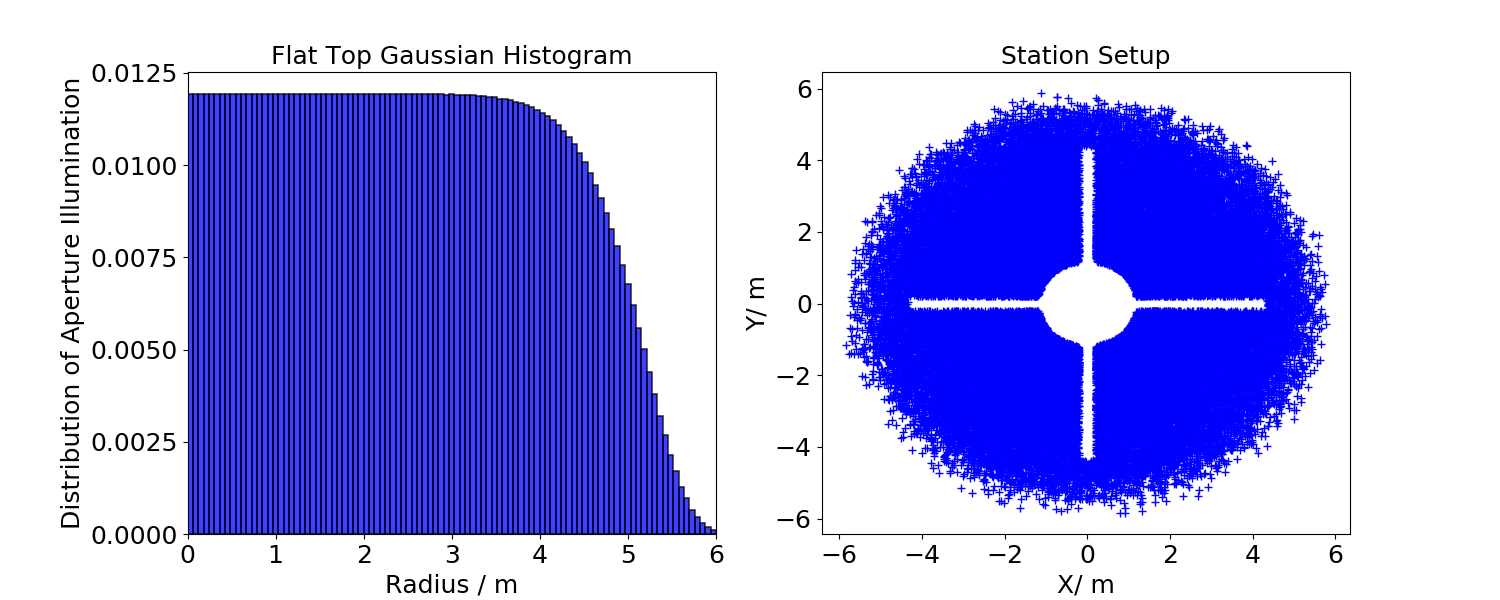
\includegraphics[width=6.0in]{c4/dhist_1} %   
%     \vspace*{1mm}
     \caption{The aperture illumination of dish-like surface is modelled using $80000$ dipoles.
        LEFT PLOT: The \enquote*{flat-top Gaussian} radial distribution of dipole positions, mimicking a realistic aperture illumination where 
        the dipoles get less dense towards the edge of the dish.
        RIGHT PLOT: The resulting 2D dipole distribution  with a mask applied to mimic aperture blockage.}        
    \label{fig:layout}
   \end{figure}
 \FloatBarrier 
%%
The parameters of the Super Gaussian distribution, $s$ and $\beta$ control the width of the distribution and the aggressiveness of the taper. 
 The values adopted in this work to produce the  radial distribution in the figure are $s = 0.82$ and  $\beta = 12.0$.\\
 %%
\noindent  We imitate the aperture blockage in point~\ref{itm:d2} by simply masking the 2D positions. This ultimately results in the dipole distribution 
shown in Fig.~\ref{fig:layout}, right. 
This dipole distribution is then fed into OSKAR as the \enquote*{station layout}. For a given set of observational parameters (in particular, pointing at zenith), 
OSKAR then computes the station primary beam response\footnote{{This takes $\approx 3 \, \rm minutes$} on a Tesla K40 GPU.}.
The resulting \emph{Jones matrix} elements are shown in Fig.~\ref{fig:jns}. 
Note how the beam pattern is broadly similar to that expected from a prime-focus dish. In particular, the first side-lobe shows the four-fold symmetry caused by the strut blockage.
The presence of the phase component in Fig.~\ref{fig:osk_im} clearly shows that the so-called ideal beam is not that perfect since we are randomly placing the dipoles in 
the KAT-7 dish-like form, hence, the norminal $X$ and $Y$ dipoles are not directly orthogonal. In effect, we get the maximum $rmse \approx 0.10 \%$ perturbed inaccuracies on 
the dish surface as reported in Fig.~\ref{fig:err}.
%
% 

\begin{figure}[H]
     \centering
     \begin{subfigure}[b]{0.7\textwidth}
         \centering
         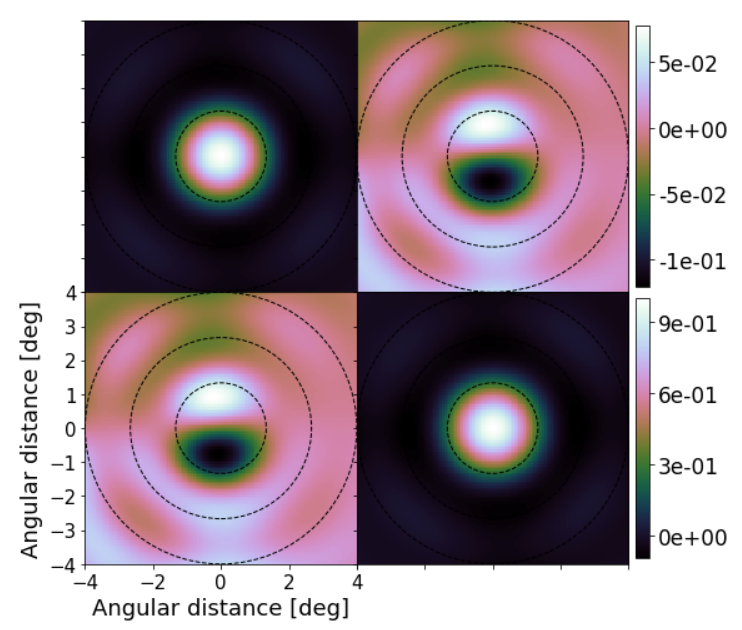
\includegraphics[width=\textwidth]{sec2jones/osk_re}
         \caption{}
         \label{fig:osk_re}
     \end{subfigure}
     \hfill
     \begin{subfigure}[b]{0.7\textwidth}
         \centering
         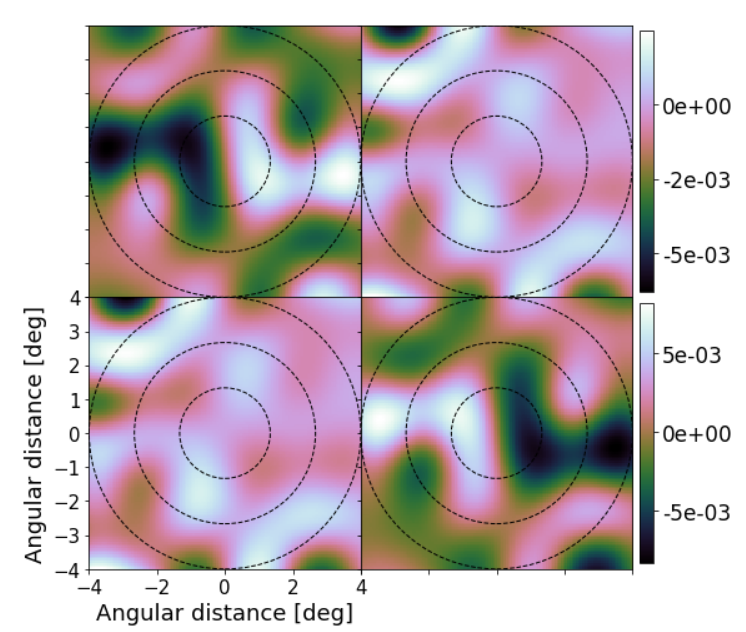
\includegraphics[width=\textwidth]{sec2jones/osk_im}
         \caption{}
         \label{fig:osk_im}
     \end{subfigure}
     \caption{Jones matrix representation of the KAT-7-like beams produced by OSKAR and shown at $1$ GHz: (a) real part (b) imaginary part. 
        The intensity of the imaginary parts increases with fewer dipoles and becomes smaller when more dipoles are used. The four panels in (a) and (b) show
        XX (top-left), XY (top-right), YX (bottom-left) and YY (bottom-right). Note that the notations X and Y denote the horizontal and vertical linear polarised beams.}\label{fig:jns}
\end{figure}
\FloatBarrier
%%
 \begin{figure}
\begin{minipage}[H]{\linewidth}
      \centering
      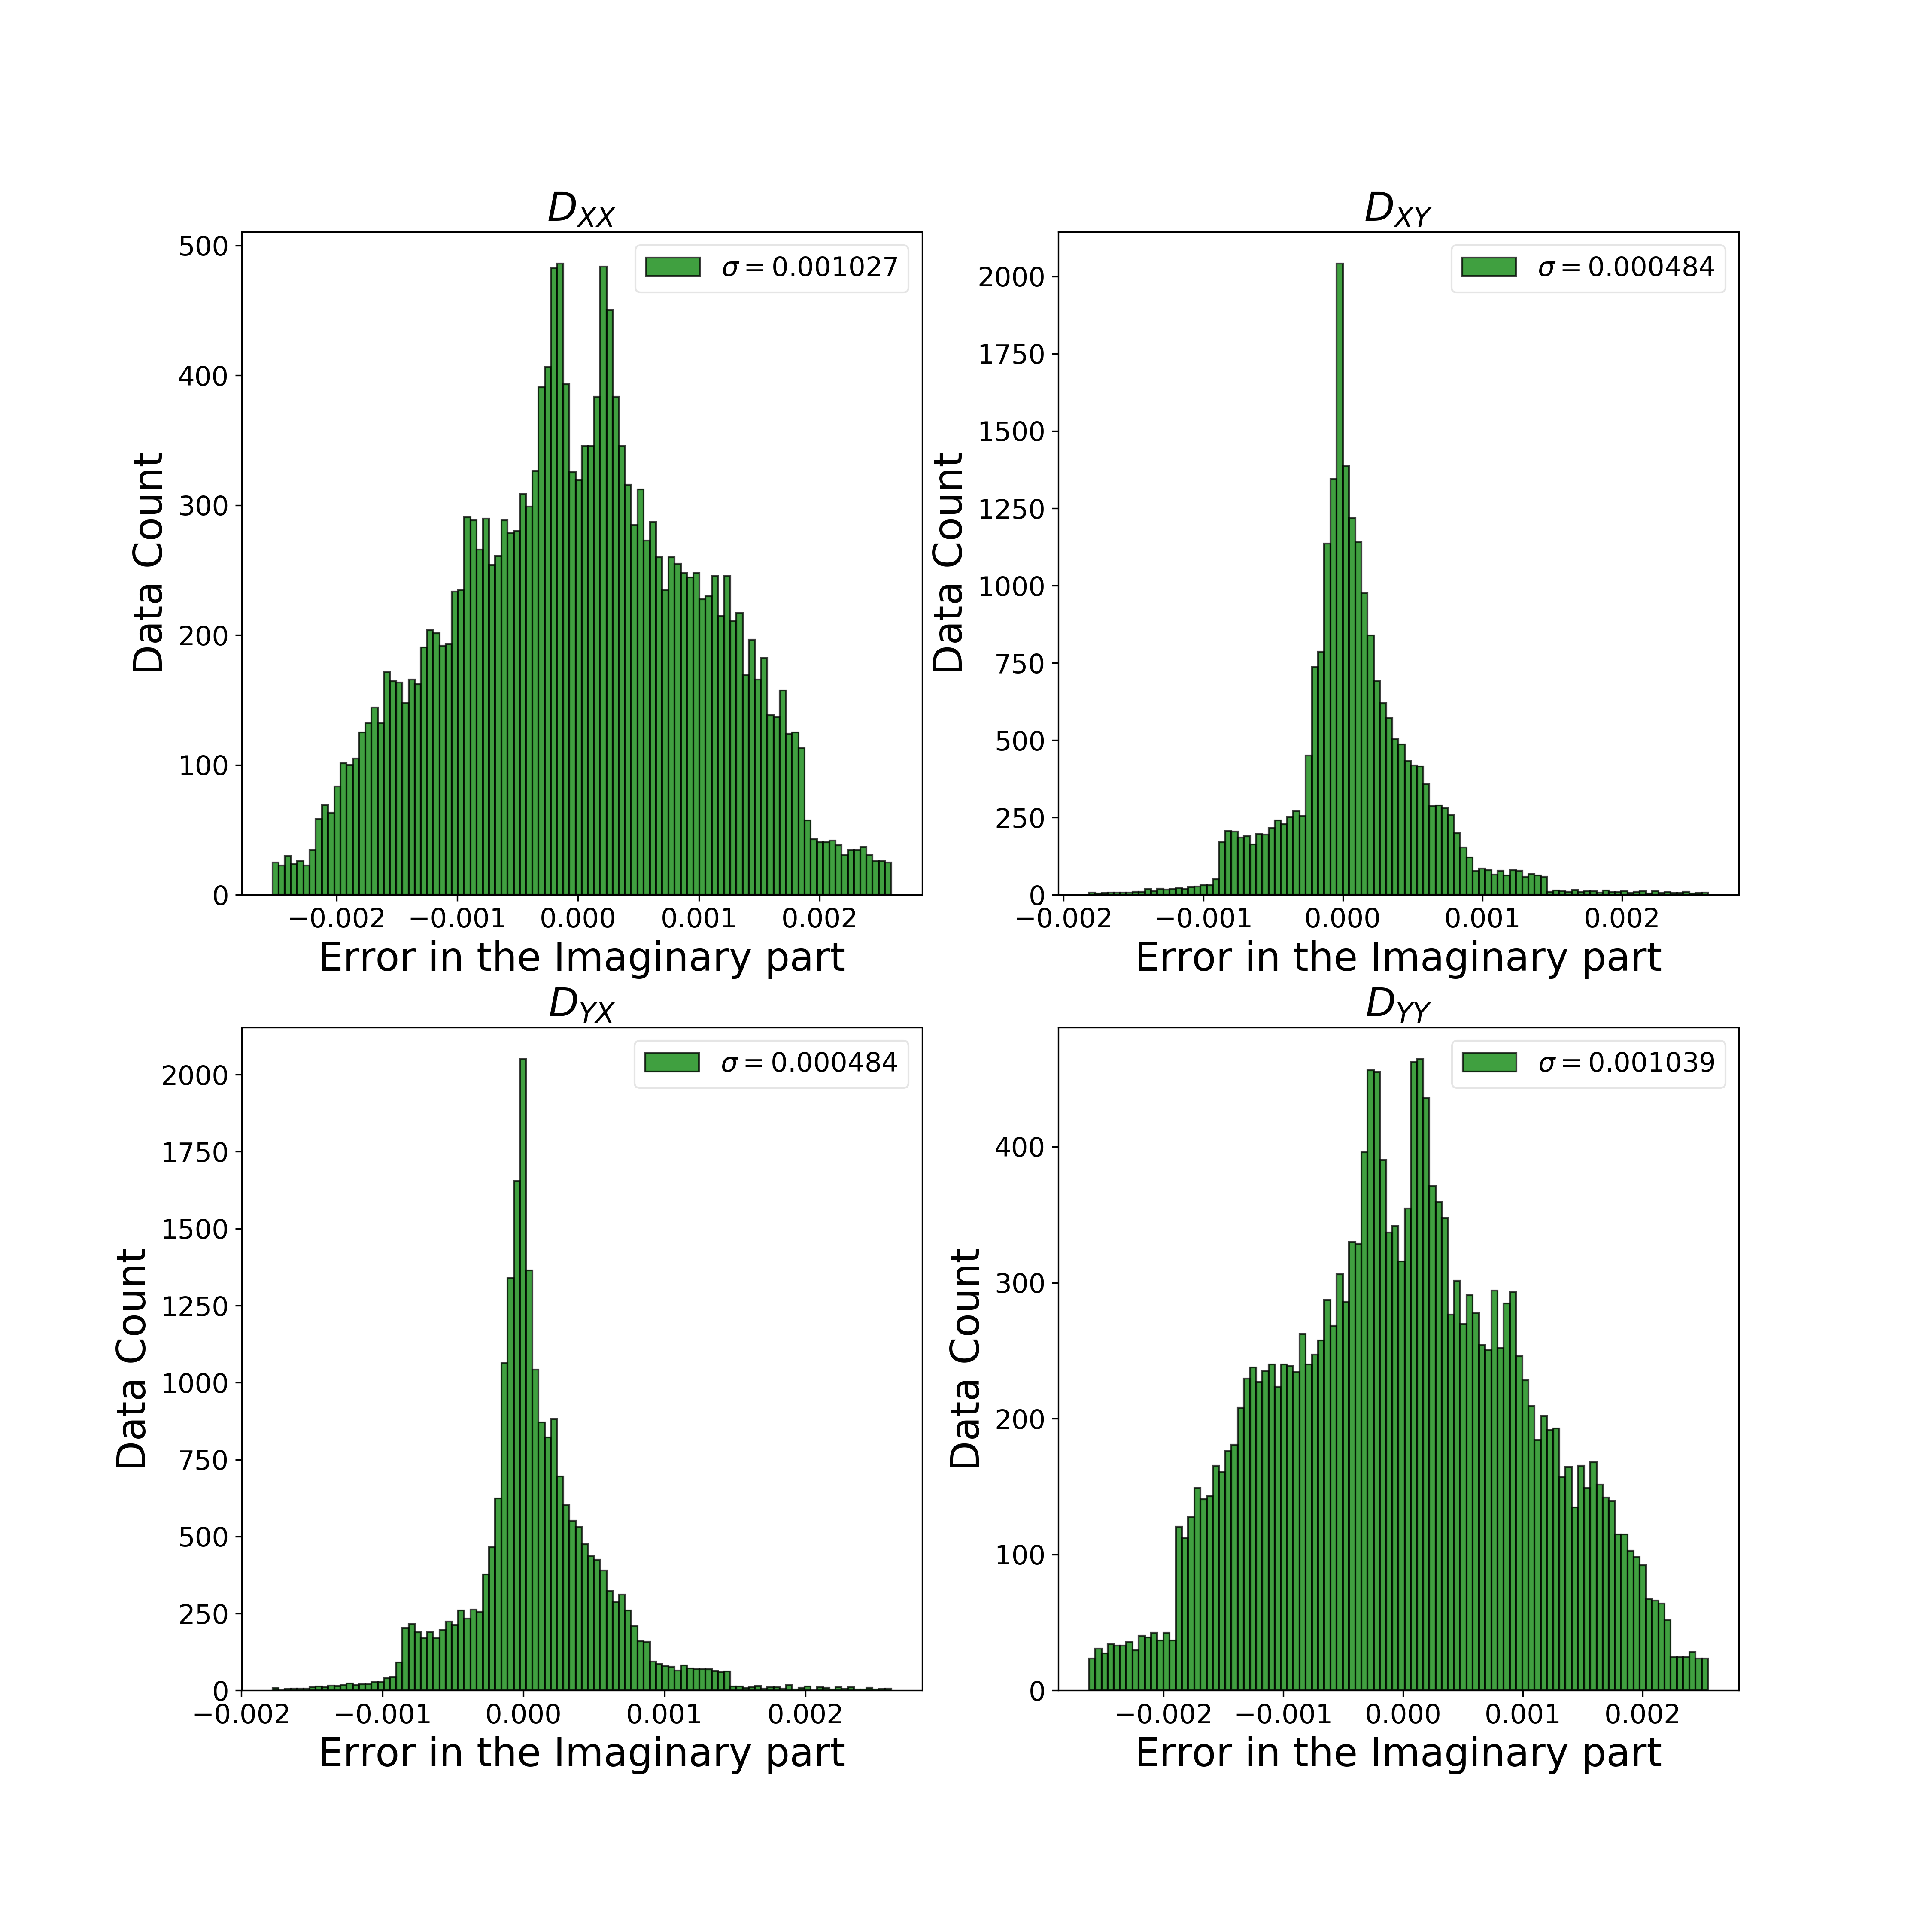
\includegraphics[width=5.8in]{sec2jones/hist_ANT1_chan0} %
    \end{minipage}
    \vspace*{-10mm}
     \caption{Histogram plots of the imaginary components in Fig.~\ref{fig:jns} showing the distribution of inaccuracies on the KAT-7 dish-like surface.}     	    \label{fig:err}
    \end{figure}
    \FloatBarrier
 
% --------------------------------------------------------------------------------------------------------------------------------

Note that the Jones \citep{1948JOSA...38..671J, 1942JOSA...32..486J} formalism, initially designed to describe optical polarization, was used 
by \cite{1996A&AS..117..137H} in radio interferometry  and further extended to direction-dependent effects by \cite{2011A&A...527A.106S}. In the next section,
we adapt the derivations of the latter two works.
%%

% +++++++++++++++++++++++++++++++++++++++++++
\subsection{Jones and Mueller matrices}       \label{sec:mueller}
% ++++++++++++++++++++++++++++++++++++++++++++
%%

An electromagnetic plane wave propagating along axis $z$ can be described, at any point in space and time, by two complex amplitudes, $e_x$ and $e_y$. 
Conventionally, we arrange these into a column vector, $\bm{e} = [e_x,e_y]^T$. A single-dish observation aims to measure the pairwise coherencies of these amplitudes:

\begin{equation}  \label{eq:pairwise}
\bm{x} = \left [ \begin{array}{c} \langle e_x e_x^* \rangle \\ \langle e_x e_y^* \rangle \\ \langle e_y e_x^* \rangle \\ \langle e_y e_y^* \rangle \end{array} \right ] =
\langle \bm{e} \circledast \bm{e}^* \rangle,
\end{equation}

\noindent where $\langle\cdot\rangle$ represents the average over a time/frequency interval, and $\otimes$ is the outer (or Kronecker) product operator.
From these measured coherencies, the Stokes parameters $IQUV$ (written as a column vector $\bm{s}$) may be derived, by definition, as \citep{1980poet.book.....B}:

\begin{equation}  \label{eq:stokes}
\bm{s} = \left [ \begin{array}{c} I \\ Q\\ U \\ V \end{array} \right ] =
\left [ \begin{array}{c} \langle e_x e_x^* \rangle + \langle e_y e_y^* \rangle \\ \langle e_x e_x^* \rangle - \langle e_y e_y^* \rangle \\
\langle e_x e_y^* \rangle + \langle e_y e_x^* \rangle \\ -\imath (\langle e_x e_y^* \rangle - \langle e_y e_x^* \rangle ) \end{array} \right ]
\end{equation}


\noindent We can rewrite this in terms of a $4\times4$ conversion matrix $\bm{S}^{-1}$ as\footnote{This follows \cite{2011A&A...527A.106S} in defining $\bm{S}$ as 
the conversion matrix between Stokes vectors and coherency vectors, $\bm{v}=\bm{Ss}$. Conversely, $\bm{S}^{-1}$ operates in the opposite direction.
Note that \cite{1996A&AS..117..137H} use $\bm{T}$ to refer to $\bm{S}^{-1}$.}:
%%

% \newpage
\begin{equation}  \label{eq:mconversion}
\bm{s} = \left[ \begin{array}{cccc}
                         1 & 0 & 0 & 1 \\
                         1 & 0 & 0 & -1 \\
                         0 & 1 & 1 & 0 \\
                         0 & -\imath & \imath & 0
                         \end{array} \right] \bm{x} = \bm{S}^{-1} \bm{x}.
\end{equation}

What the instrument actually measures is a set of pairwise correlations between two voltages induced by the EM field on two orthogonal mode feeds, $v_a$ and $v_b$. 
The Jones formalism assumes that these are linearly related to the EM field (i.e. that all signal propagation effects are linear). 
This can be written as $\bm{v}=\bm{J} \bm{e}$, where $\bm{v}$ is a column vector of the two voltages, and the $2\times 2$ \emph{Jones matrix} $\bm{J}$ 
describes signal propagation. The \emph{measured} coherency $\bm{x}'$ can then be written as:

% \newpage
\begin{equation}
\bm{x}' = \langle \bm{v} \circledast \bm{v}^* \rangle = (\bm{J} \circledast \bm{J}^* ) \langle \bm{e} \circledast \bm{e}^* \rangle =
(\bm{J} \circledast \bm{J}^* ) \bm{x},
\end{equation}

\noindent and the measured Stokes parameter vector $\bm{s}'$ relates to the original Stokes vector via the so-called \emph{Mueller matrix} $\bm{M}$:

\begin{equation} \label{eq:simpl}
\bm{s}' = \bm{M} \bm{s} = \bm{S}^{-1} (\bm{J} \circledast \bm{J}^* ) \bm{S} \bm{s}
\end{equation}

\noindent For the purposes of this work, we ignore all propagation effects except the primary beam. 
%%
   
\noindent Therefore, expanding the Jones terms in Equation~\ref{eq:simpl}, we can measure the full elements of $\bm{M}$, thus:
%%
\begin{eqnarray} \bm{J} \circledast \bm{J}^* = \left( \begin{array}{cccc}
                         j_{\rm xx}\,j_{\rm xx}^* & j_{\rm xx}\,j_{\rm xy}^* & j_{\rm xy}\,j_{\rm xx}^* & j_{\rm xy}\,j_{\rm xy}^* \\
                         j_{\rm xx}\,j_{\rm yx}^* & j_{\rm xx}\,j_{\rm yy}^*  & j_{\rm xy}\,j_{\rm yx}^* & j_{\rm xy}\,j_{\rm yy}^* \\
                         j_{\rm yx}\,j_{\rm xx}^* & j_{\rm yx}\,j_{\rm xy}^* & j_{\rm yy}\,j_{\rm xx}^* & j_{\rm yy}\,j_{\rm xy}^* \\
                         j_{\rm yx}\,j_{\rm yx}^* & j_{\rm yx}\,j_{\rm yy}^* & j_{\rm yy}\,j_{\rm yx}^* & j_{\rm yy}\,j_{\rm yy}^*
                         \end{array} \right) \label{eq:fr19} \end{eqnarray}
                         %
                         
\noindent  If we substitute Equation~\ref{eq:fr19} into~\ref{eq:simpl}, we can then expand $\bm{M}$ in terms of Jones matrix elements:
%
\begin{subequations}\label{eq:fr20}
  \begin{align}
  m_{\rm II} & = (j_{\rm xx}j_{\rm xx}^{*}\, + j_{\rm xy}j_{\rm xy}^{*}\, + j_{\rm yx}j_{\rm yx}^{*}\, + j_{\rm yy}j_{\rm yy}^{*})/2  	\label{eq:fr20a}\\
  m_{\rm IQ} & = (j_{\rm xx}j_{\rm xx}^{*}\, - j_{\rm xy}j_{\rm xy}^{*}\, + j_{\rm yx}j_{\rm yx}^{*}\, - j_{\rm yy}j_{\rm yy}^{*})/2 	 \label{eq:fr20b}\\
  m_{\rm IU} & = (j_{\rm xx}j_{\rm xy}^{*}\, + j_{\rm xy}j_{\rm xx}^{*}\, + j_{\rm yx}j_{\rm yy}^{*}\, + j_{\rm yy}j_{\rm yx}^{*})/2  	\label{eq:fr20c}\\
  m_{\rm IV} & = i(j_{\rm xx}j_{\rm xy}^{*}\, + j_{\rm yx}j_{\rm yy}^{*}\, - j_{\rm xy}j_{\rm xx}^{*}\, - j_{\rm yy}j_{\rm yx}^{*})/2  	\label{eq:fr20d}\\
  m_{\rm QI} & = (j_{\rm xx}j_{\rm xx}^{*}\, + j_{\rm xy}j_{\rm xy}^{*}\, - j_{\rm yx}j_{\rm yx}^{*}\, - j_{\rm yy}j_{\rm yy}^{*})/2  	\label{eq:fr20e}\\
  m_{\rm QQ} & = (j_{\rm xx}j_{\rm xx}^{*}\, - j_{\rm xy}j_{\rm xy}^{*}\, - j_{\rm yx}j_{\rm yx}^{*}\, + j_{\rm yy}j_{\rm yy}^{*})/2  	\label{eq:fr20f}\\
  m_{\rm QU} & = (j_{\rm xx}j_{\rm xy}^{*}\, + j_{\rm xy}j_{\rm xx}^{*}\, - j_{\rm yx}j_{\rm yy}^{*}\, - j_{\rm yy}j_{\rm yx}^{*})/2 	\label{eq:fr20g}\\
  m_{\rm QV} & = i(j_{\rm xx}j_{\rm xy}^{*}\, - j_{\rm yx}j_{\rm yy}^{*}\, - j_{\rm xy}j_{\rm xx}^{*}\, - j_{\rm yy}j_{\rm yx}^{*})/2 	\label{eq:fr20h}\\
  m_{\rm UI} & = (j_{\rm xx}j_{\rm yx}^{*}\, + j_{\rm yx}j_{\rm xx}^{*}\, + j_{\rm xy}j_{\rm yy}^{*}\, + j_{\rm yx}j_{\rm xy}^{*})/2 	\label{eq:fr20i}\\
  m_{\rm UQ} & = (j_{\rm xx}j_{\rm xy}^{*}\, - j_{\rm xy}j_{\rm xx}^{*}\, + j_{\rm yx}j_{\rm yy}^{*}\, + j_{\rm yy}j_{\rm yx}^{*})/2  	\label{eq:fr20j}\\
  m_{\rm UU} & = (j_{\rm xx}j_{\rm yy}^{*}\, + j_{\rm yy}j_{\rm xx}^{*}\, + j_{\rm xy}j_{\rm yx}^{*}\, + j_{\rm yx}j_{\rm xy}^{*})/2 	 \label{eq:fr20k}\\
  m_{\rm UV} & = i(j_{\rm xx}j_{\rm yy}^{*}\, + j_{\rm yx}j_{\rm xy}^{*}\, - j_{\rm yy}j_{\rm xx}^{*}\, - j_{\rm xy}j_{\rm yx}^{*})/2 	\label{eq:fr20l}\\
  m_{\rm VI} & = i(-j_{\rm xx}j_{\rm yx}^{*}\, + j_{\rm yx}j_{\rm xx}^{*}\, - j_{\rm xy}j_{\rm yy}^{*}\, + j_{\rm yy}j_{\rm xy}^{*})/2  	\label{eq:fr20m}\\
  m_{\rm VQ} & = i(-j_{\rm xx}j_{\rm yx}^{*}\, + j_{\rm yx}j_{\rm xx}^{*}\, + j_{\rm xy}j_{\rm yy}^{*}\, - j_{\rm yy}j_{\rm xy}^{*})/2 	\label{eq:fr20n}\\
  m_{\rm VU} & = i(-j_{\rm xx}j_{\rm yy}^{*}\, + j_{\rm yy}j_{\rm xx}^{*}\, - j_{\rm xy}j_{\rm yx}^{*}\, + j_{\rm yx}j_{\rm xy}^{*})/2 	 \label{eq:fr20o}\\
  m_{\rm VV} & = (j_{\rm xx}j_{\rm yy}^{*}\, - j_{\rm yx}j_{\rm xy}^{*}\, + j_{\rm yy}j_{\rm xx}^{*}\, - j_{\rm xy}j_{\rm yx}^{*})/2  	\label{eq:fr20p} 
 \end{align}
%  \phantom{\hspace{1cm}} 
\end{subequations}
%
The sixteen elements in Equations~\ref{eq:fr20a} to~\ref{eq:fr20p} are the complete PBs of a radio telescope (as shown in Fig.~\ref{fig:truosk}) produced from the complex beams 
(see Fig.~\ref{fig:jns}). The DD effect of the PB will cause each element in Equation~\ref{eq:fr20} to produce different matrices. 
If we substitute the elements in Equation~\ref{eq:fr20} into Equation~\ref{eq:simpl}, we get the measured Stokes parameters in Equation~\ref{eq:fr21}:

\begin{eqnarray} \left( \begin{array}{c}
                         S'_{I}\\
                         S'_{Q}\\
                         S'_{U}\\
                         S'_{V}
                        \end{array} \right) =
\left( \begin{array}{cccc}
                        m_{II} & m_{IQ} & m_{IU} & m_{IV} \\
                        m_{QI} & m_{QQ} & m_{QU} & m_{QV} \\
                        m_{UI} & m_{UQ} & m_{UU} & m_{UV} \\
                        m_{VI} & m_{VQ} & m_{VU} & m_{VV} \end{array} \right)                     
                     \left( \begin{array}{c}
                         S_{I}\\
                         S_{Q}\\
                         S_{U}\\
                         S_{V}
                        \end{array} \right)  \label{eq:fr21}
\end{eqnarray} 

% %%
% \begin{equation}
% \bm{s}'_\mathrm{tot} = \iint\limits_{lm} \bm{M}(l,m) \bm{s}(l,m) \mathrm{d}l \mathrm{d}m,
% \end{equation}
% 
% \noindent where the integration is, in principle, over the entire celestial sphere, but in practice, since the Mueller matrix becomes negligibly 
% small outside of a certain FoV, it can be replaced by a 2D integral over the tangent plane $lm$.
% %%


Note the physical meaning of the matrix elements. The on-diagonal terms of the Jones matrix describe the sensitivity of each feed, as a function of direction, to its matched 
EM field component. The off-diagonal terms describe leakage, i.e. the sensitivity of the feed to the nominally orthogonal EM field component. This leakage is due to mechanical
and electronic imperfections in the antennas and feeds. The diagonal terms of the Mueller matrix describe the sensitivity of the measured Stokes $IQUV$ components to their true counterparts, 
as a function of direction. The off-diagonal terms describe spurious leakage between the measured Stokes components. We can schematically write this as;
% \newpage
$$ \bm{M}  =
\left[ \begin{array}{cccc}
  I \rightarrow I' & Q \rightarrow I' & U \rightarrow  I' & V \rightarrow  I' \\
  I \rightarrow Q' & Q \rightarrow Q' & U \rightarrow  Q' & V \rightarrow  Q'\\
  I \rightarrow U' & Q \rightarrow U' & U \rightarrow  U' & V \rightarrow  U'\\
  I \rightarrow V' & Q \rightarrow V' & U \rightarrow  V' & V \rightarrow  V'
\end{array} \right]
$$


\begin{figure}
  \centering
  \begin{minipage}[H]{\linewidth}
     \begin{subfigure}[b]{0.8\textwidth}
      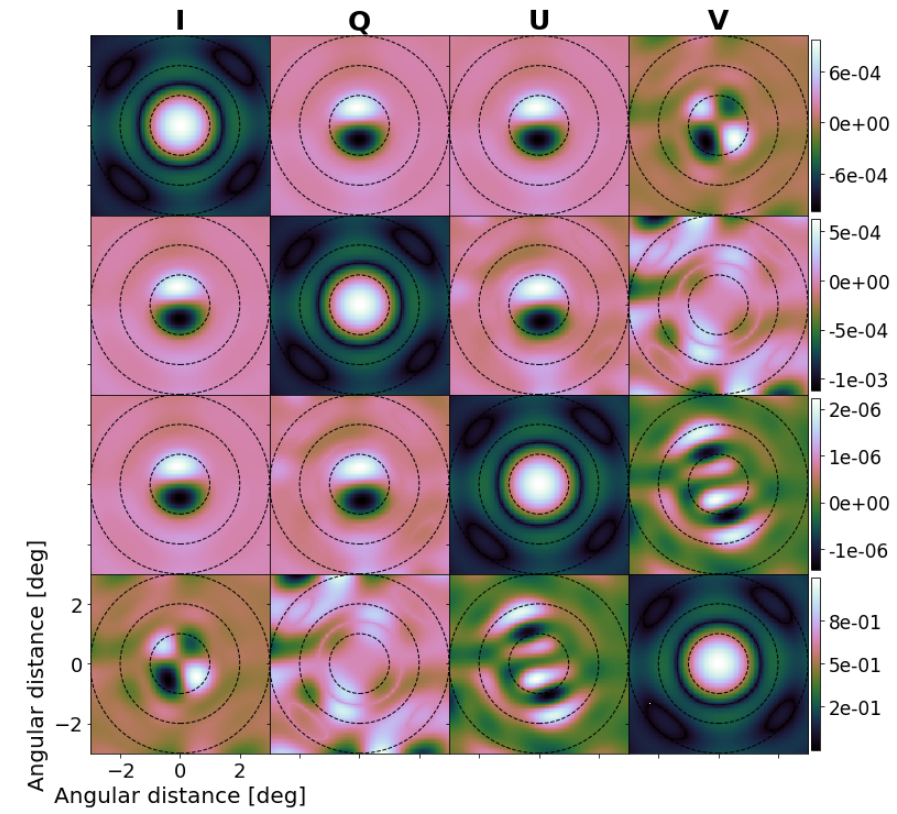
\includegraphics[width=\textwidth]{sec2oskbms/osk_trumueller}
                \caption{}
                \label{fig:truosk1}
        \end{subfigure}
        \qquad
        \begin{subfigure}[b]{0.8\textwidth}
 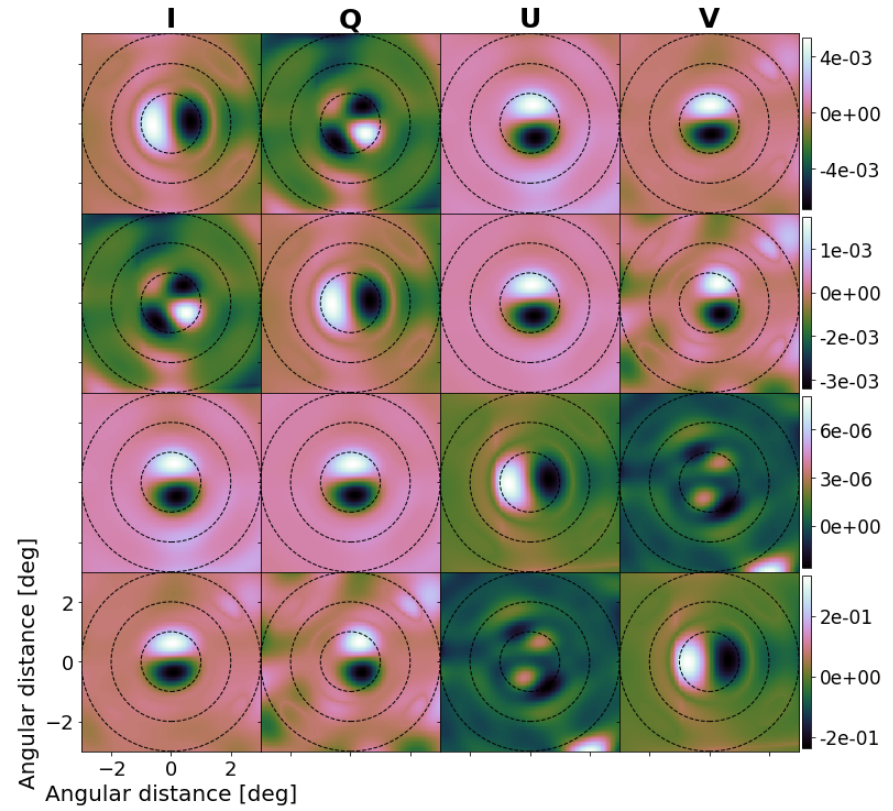
\includegraphics[width=\textwidth]{sec2oskbms/osk_tru-gpmueller}
                \caption{}
               \label{fig:truosk2}
        \end{subfigure}
%         
\end{minipage}
  \end{figure}
  \FloatBarrier
  
 %% 
  \begin{figure}
\ContinuedFloat
\centering
 \begin{minipage}[H]{\linewidth}
\begin{subfigure}[b]{0.8\textwidth}
      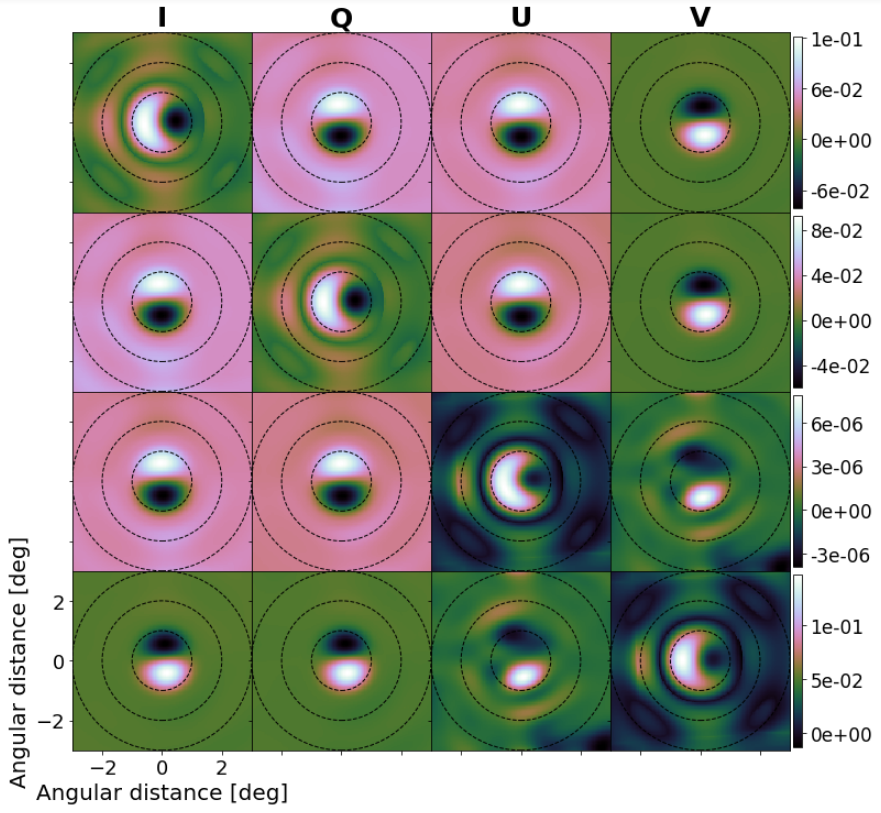
\includegraphics[width=\textwidth]{sec2oskbms/osk_tru-xymueller}
                \caption{}
                \label{fig:truosk3}
        \end{subfigure}
        \qquad
        \begin{subfigure}[b]{0.8\textwidth}
         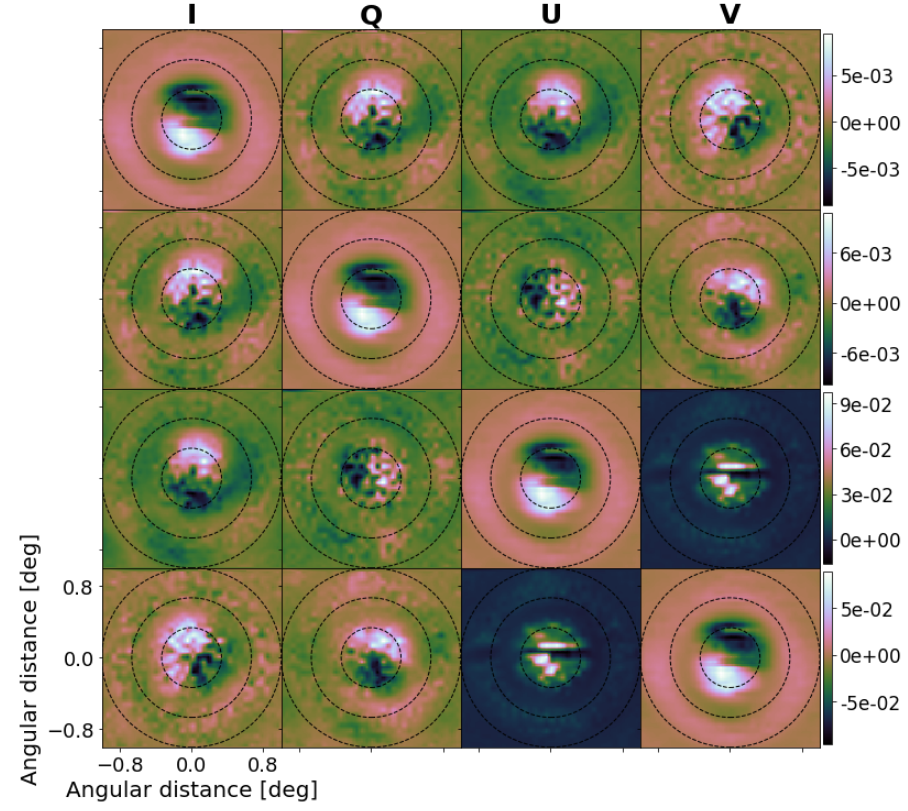
\includegraphics[width=\textwidth]{sec2realbms/vla-diffmueller}
                \caption{}
               \label{fig:truosk4}
        \end{subfigure}
         \end{minipage}
    \caption{\small{ Mueller matrix representations of full polarization beams produced at $1\, \mathrm{GHz}$
    (a) $4 \times 4$ images of KAT-7 uncorrupted OSKAR beams.
    (b) Fractional differences between the uncorrupted OSKAR beams in Fig.~\ref{fig:truosk1} and the gain and phase error beams in appendix~\ref{fig:A1a} 
     (c) Fractional differences between uncorrupted OSKAR beams in Fig.~\ref{fig:truosk1} and the dipole orientation error beams in  appendix~\ref{fig:A1b}.
     (d) Fractional differences between VLA holography measured beams in   Figs.~\ref{fig:A2a} and~\ref{fig:A2b}.}}      
	    \label{fig:truosk}
  \end{figure}
  \FloatBarrier

% +++++++++++++++++++++++++++++++++++++++++++
\subsection{Primary Beam Perturbation}       \label{sec:perturb}
% ++++++++++++++++++++++++++++++++++++++++++++
%%

For the purpose of this research, we try to introduce some distortions on the simulated OSKAR beams for IM experiment.
The first type is to corrupt both the gain and phase of the beam in a systematic manner. Here, we can do this with OSKAR by simulating
the gain and phase of each element so that the weight of the beamformer $W_{\rm B}$ at a particular time $t$, for a given pointing direction $(\vartheta_{\rm B}, \varphi_{\rm B})$
and dipole locations $(\upsilon_{\rm 1}, \upsilon_{\rm 2}, \upsilon_{\rm 3})$ is given in \citep{ansah2018simulations} as:

% EQ11
\begin{equation} W_{\rm B} (\bm{\upsilon}) =  (G_{\rm B}^{ 0} + G_{\rm B}^{error}) W_{B}^{geo}(\bm{\upsilon})\mathrm{e}^{j\left(\varphi_{\rm B}^{0} + \varphi_{\rm B}^{error} \right)} \label{eq:q11} \end{equation} 
%%


% The modelled beams produced in this chapter are corrupted with two kinds of errors. The first error type is the introduction of systematic and time-variable 
% gain and phase errors. The nominal purpose of this in OSKAR is to simulate per-element gain and phase error before the beamformer, so that the beam-forming weight $B^{w}$, 
% for a particular beam direction $(\theta_{bm}, \phi_{bm})$, with dipole position $(x, y, z)$ and time $t$ becomes;%%
% %%
% % EQ11
% \begin{equation} W_{\rm B} =  W_{B}^{geo}(u)(G_{0} + G_{error})\exp(j\left[\phi_{0} + \phi_{error}\right]) \label{eq:q11} \end{equation} 
% %%
\noindent The parameters  $\bm{\upsilon} = (\vartheta_{\rm B}, \varphi_{\rm B}, \upsilon_{\rm 1}, \upsilon_{\rm 2}, \upsilon_{\rm 3}, t)$, 
$G_{\rm B}^{error}$ and $\varphi_{\rm B}^{error}$ use the Gaussian function to generate deterministic random numbers at step-time $t$. We then combine these
parameters with $G_{\rm B}^{ 0}$ (the gain), $\varphi_{\rm B}^{0}$ (phase) and the geometrical kernel function $W_{B}^{geo}$, to obtain the array factor for beam evaluation.
%%
For the purpose of our \enquote{disk-like} simulation, we introduced $5^\circ$ 
phase error and $10 \%$ gain error into the beam-forming weight to distort the beams as shown in Fig.~\ref{fig:A1a}. These types of errors represent imperfections 
in the parabolic reflector surface (which, in real life, result in amplitude and phase errors over the aperture).
%%
The second perturbation is to introduce positional errors per element. Note that for ideal situation, both dipoles $(x,y)$ are orthogonal and the angular differences 
will be zero. However, displacing the dipoles from its nominal positions ($\sim 1^\circ$) will definitely produce an angular difference of being greater than zero, hence, creating a
systematic error in the feed angle and the effect of this is presented in  Fig.~\ref{fig:A1b}. Here, what we do is to indicate the Euler angles of the feeds of the nominal $x$ and $y$ dipoles in each station directory. These angles depict the differences from zero, since in the ideal case  both dipoles are expected to be  orthogonal and in the plane of the station platform.
%%
Figs.~\ref{fig:truosk2} and~\ref{fig:truosk3} 
show the beam errors produced by computing the differences between the true modelled beams in Fig.~\ref{fig:truosk1} and the two distorted beams in Figs.~\ref{fig:A1a} 
and~\ref{fig:A1b} respectively. The on-diagonal components of these beam errors represent the residual leakages and the off-diagonals show the residual systematic leakages. 
The maximum residual leakages produced in Figs.~\ref{fig:truosk2} and~\ref{fig:truosk3} are $\simeq 20 \%$ and $10 \%$ respectively.
%%

%%
Another thing that we considered in this work is to apply the JVLA holography beams to measure the degree of beam perturbation. The numerical scheme used to generate 
the JVLA beams in Figs.~\ref{fig:A2a} and~\ref{fig:A2b} is described in the EVLA Memo \citep{2015Rick} which involves the use of Fourier transform to determine the far-field 
beam pattern of an antenna. Fig.~\ref{fig:truosk4} is the residual error of the JVLA beams, producing $\simeq 10 \%$ leakage. Therefore, the systematic leakage in the holography
beams indicates that the simulated perturbations introduced in the OSKAR beams  are actually practical. 
%%

Now that we are abreast with the model of the instrument, we continue to show how we apply these beams to the simulated full-sky maps discussed in Chapter~\ref{Chapter3}.
%%

\section{Convolution of Foreground Maps}    \label{sec:convolution}
%%%

 %
Mathematically, convolution is an  operator that interpolates two expressions $\varUpsilon_{\rm \alpha}$ and $\varUpsilon_{\rm \beta}$ 
to produce a third function $\chi$ 
that is typically viewed as a modification of one of the original functions. Consider $C_{v}(\varsigma)$ to be the convolution of $ \Psi_{\rm \alpha}(\varsigma)$
with $ \Psi_{\rm \beta}(\varsigma)$, then its Fourier pair  $\chi(\nu)$, is the product of $\varUpsilon_{\rm \alpha} (\nu)$ and $\varUpsilon_{\rm \beta} (\nu)$ which define the 
Fourier pairs of $ \Psi_{\rm \alpha}(\varsigma)$ and $ \Psi_{\rm \beta}(\varsigma)$ respectively. Thus,
%
% EQ1
\begin{equation}  \Psi_{\rm \alpha}(\varsigma)\, \odot\, \Psi_{\rm \beta}(\varsigma) \, \rightleftharpoons \, \varUpsilon_{\rm \alpha} (\nu). \varUpsilon_{\rm \beta} (\nu) \label{eq:u31} \end{equation}
%

\noindent where the symbol $\odot$ denotes the convolution operator. By definition,
%% EQ2
\begin{equation}
 \begin{aligned}
  C_{v}(\varsigma) &=  \Psi_{\rm \alpha}(\varsigma) \,\odot \,  \Psi_{\rm \beta}(\varsigma)\\
  &= \int_{- \infty}^{\infty}\,  \Psi_{\rm \alpha}(\varsigma')  \Psi_{\rm \beta}(\varsigma - \varsigma') \mathnormal{d\varsigma} 
  \end{aligned}
  \label{eq:u32}
\end{equation}
%
Taking the Fourier transform of both sides in Equation~\ref{eq:u32}, we get:
% % EQ3
\begin{equation}
\begin{aligned}
 \chi(\nu) &= \int_{- \infty}^{\infty} C_{v}(\varsigma)\mathnormal{e}^{-2\pi j \nu \varsigma}\mathnormal{d\varsigma}\\
 &= \int_{- \infty}^{\infty} \int_{- \infty}^{\infty} \,
  \Psi_{\rm \alpha}(\varsigma')  \Psi_{\rm \beta}(\varsigma - \varsigma')\mathnormal{e}^{-2\pi j \nu \varsigma}\mathnormal{d\varsigma'\, d\varsigma}
 \end{aligned}
   \label{eq:u33}
\end{equation}
%
Let $ y = \varsigma - \varsigma' \, \Rightarrow \, \mathnormal{dy} = \mathnormal{d\varsigma} $
%% EQ4
\begin{equation}
  \chi(\nu) =  \int_{- \infty}^{\infty} \int_{- \infty}^{\infty} \,   \Psi_{\rm \alpha}(\varsigma')  \Psi_{\rm \beta}(y)\mathnormal{e}^{-2\pi j\nu(\varsigma' + y)}
  \mathnormal{d\varsigma'} \mathnormal{dy}
   \label{eq:u34}
\end{equation}
%
Equation~\ref{eq:u34} can therefore be separated to give:

% EQ5
\begin{equation}
 \begin{aligned}
  \chi(\nu)  & =\,  \int_{- \infty}^{\infty} \,   \Psi_{\rm \alpha}(\varsigma')\mathnormal{e}^{-2\pi j \nu \varsigma'} \mathnormal{d\varsigma'}.
  \int_{- \infty}^{\infty} \,  \Psi_{\rm \beta}(y)\mathnormal{e}^{-2\pi j \nu y} \mathnormal{dy} \\
   & =\,  \varUpsilon_{\rm \alpha}(\nu). \varUpsilon_{\rm \alpha}(\nu)
\end{aligned}
\label{eq:u35}
\end{equation}
%
Expressing the general definition in Equation~\ref{eq:u35} into $\rm 2D$ discrete form, we have:

%% EQ6
 \begin{equation}
   \begin{aligned}
   \chi(\nu_{\rm \alpha}, \nu_{\rm \beta}) &=   \Psi_{\rm \alpha}(\nu_{\rm \alpha}, \nu_{\rm \beta}) \,\odot \Psi_{\rm \beta}(\nu_{\rm \alpha}, \nu_{\rm \beta}) \\ 
  &= \, \sum_{m = - \infty}^{\infty} \sum_{n = - \infty}^{\infty} \,   \Psi_{\rm \alpha} (m - \nu_{\rm \alpha}, n - \nu_{\rm \beta}) \Psi_{\rm \beta}(m, n)
  \end{aligned}
\label{eq:u36} 
\end{equation}
%
In Equation~\ref{eq:u36}, the values $  \chi(\nu_{\rm \alpha}, \nu_{\rm \beta})$ of the discrete function $ \chi$ for any particular $ (\nu_{\rm \alpha}, \nu_{\rm \beta})$ follows by multiplying
each value $ \Psi_{\rm \beta}(m, n)$ of the discrete function $ \Psi_{\rm \beta}$ with a kernel function $ \Psi_{\rm \alpha} (m - \nu_{\rm \alpha}, n - \nu_{\rm \beta})$
between a particular 
$ (\nu_{\rm \alpha}, \nu_{\rm \beta})$ and varying $(m, n)$ where, $(- \infty \, < \, m, \, n \, <  \, + \infty)$. Thus, each value $  \chi(\nu_{\rm \alpha}, \nu_{\rm \beta})$ of the function 
$ \chi$ is a weighted mean of the values $ \Psi_{\rm \beta}(m, n)$ with weights $ \Psi_{\rm \alpha} (m - \nu_{\rm \alpha}, n - \nu_{\rm \beta})$ defined by the function
$ \Psi_{\rm \alpha}$. In this chapter, we apply similar approach to simulate the foreground of the sky.
To perform an IM experiment, the radio telescope(s) is pointed at different patches of the sky so that the instrument can measure the overall
intensity emerging from patches from the autocorrelation of the radio signal, as a function of frequency. In order to emulate this observation 
technique in our IM simulation, the discrete convolution in Equation~\ref{eq:q13} is used to measure the intensities of the full sky synchrotron 
maps in Fig.~\ref{fig:f1000}. Let $(\theta, \phi)$ denote the celestial coordinates of the foregrounds of the sky, such that $\bm{B}$ are the fully
polarised beams  and $\bm{f_{\rm sky}}$ are the foregrounds of the sky. We can then model the convolved foregrounds to be: 
 
%% EQ7
\begin{equation}	\label{eq:q13}  
\begin{aligned}  
  \bm{F^{conv}}(\theta, \phi) & =\,  \bm{B}(\theta, \phi) \, \odot \bm{f_{\rm sky}}(\theta, \phi) \\
  & = \sum_{ (\theta', \phi') = \,\lfloor \, (\theta, \phi) \, \rceil} \!\!\!  
  \bm{B}(\theta' - \theta, \phi' - \phi).\bm{f_{\rm sky}}(\theta', \phi')
\end{aligned} 
  \end{equation}
 % 
 
\noindent where  $ (\theta', \phi') \leq npix$ and the symbol $\lfloor \, \rceil$ denotes the nearest pixels. The measured foreground
pixel values $\bm{ F^{conv}}(\theta, \phi)$ of the discrete function $\bm{F^{conv}}$ for any particular $ (\theta, \phi)$ follows by 
multiplying each foreground pixel value $\bm{f_{\rm sky}}(\theta, \phi)$ of the discrete function $\bm{f_{\rm sky}}$ with a beam  $\bm{B}(\theta' - \theta, \phi' - \phi)$
between a particular $ (\theta', \phi')$ and varying $(\theta, \phi)$. Thus, each pixel value $\bm{ F^{conv}}(\theta, \phi)$ of the function $\bm{F^{conv}}$ is 
a weighted mean of the pixel values $\bm{f_{\rm sky}}(\theta, \phi)$ with weights $\bm{B}(\theta' - \theta, \phi' - \phi)$ defined by the function $\bm{B}$.

The convolution technique in Equation~\ref{eq:q13} is implemented in this work using the {\tt HEALPix} query disc function (Python package). 
This function is applied on the {\tt HEALPix} map (the full-sky map) with $Nside = 512$ to query all the nearby pixels that fall within the primary beamwidth for every pointing.
These query pixels are then convolved with the corresponding pixel values in the beam. So for each pointing, we get different query pixels even though there can be overlapping pixels
like the rings shown in Fig.~\ref{fig:implota}, as you point the beam to the next direction. To measure the exact intensity of the foreground, the convolved {\tt HEALPix} map is normalised by the power beam (Stokes I). For instance, in Equation~\ref{eq:q13}, if we let $\bm{B}$ to be the complete beams in Fig.~\ref{fig:truosk1}  and then replace $\bm{f_{\rm sky}}$ with Fig.~\ref{fig:f1000}, we generate $\bm{ F^{conv}}$ as shown in Fig.~\ref{fig:fgTrCnv}. We repeat the procedure, using the beams in Figs.~\ref{fig:A1a} and~\ref{fig:A1b} to obtain perturbed maps.  Similarly, doing same for the JVLA beams in Figs.~\ref{fig:A2a} and~\ref{fig:A2b}, we produce their corresponding  measured sky maps. In Fig.~\ref{fig:fgTrCnv}, we can observe that the spatial representation of the inclining maps from left to right are retained as that of the initial foreground images displayed in Fig.~\ref{fig:f1000}. This happens when we convolve the sky maps with the gain terms (i.e. $m_{\rm II}, m_{\rm QQ}, m_{\rm UU}$).

%%

In performing IM,  we are mostly curious about the absolute intensity of the foreground. This can be done by transforming the spatial representation of the convolved sky maps 
into spherical harmonics in order to estimate the power spectrum in a scale of moments ($l$). The next section presents the angular power spectrum described in \citep{ansah2018simulations}.
% actually interested in, is to measure the total intensity of a signal. Therefore, in Section~\ref{sec:spectrum},
%  we present a mathematical model of the convolved power spectrum using the angular power spectrum approach to describe the spatial distribution of the measured foregrounds in a spherical harmonic domain
%%

\begin{figure}
\centering
\begin{minipage}[H]{\linewidth}
       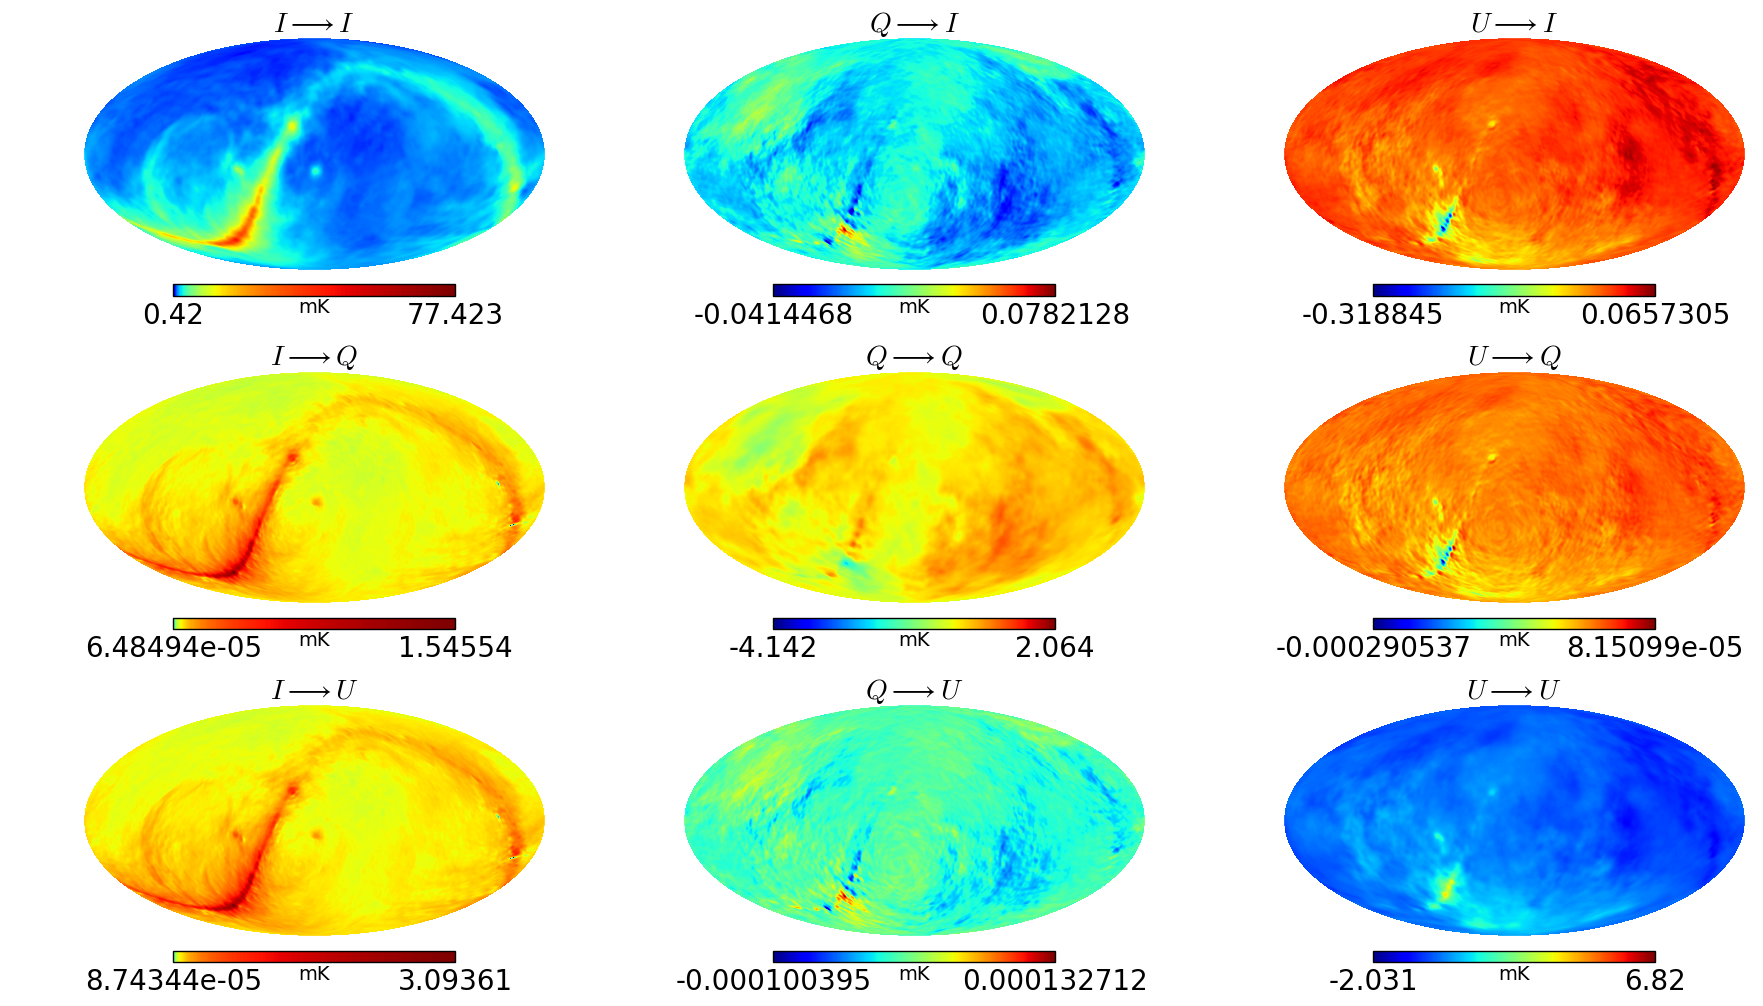
\includegraphics[width=6.6in]{sec3gp_conv/osk_Tr1}
      \end{minipage}
    \caption{Convolved full-sky polarization maps using the non-distorted OSKAR beams. 
    For example, we used the $m_{\rm II}$ beam in Fig.~\ref{fig:truosk1} to convolve Stokes $I$ in Fig.~\ref{fig:f1000} and produce the convolved map $I \rightarrow I$ , 
    then we used $m_{\rm QI}$ beam to convolve Stokes $Q$ to obtain the convolved map $Q \rightarrow I$, also, using the $m_{\rm UI}$ beam to convolve Stokes $U$ we produced the convolved map $U \rightarrow I$. The other convolved maps are produced in the same manner using their respective beams.} \label{fig:fgTrCnv}
\end{figure}
\FloatBarrier


% 
\subsection{Angular Power Spectrum}    \label{sec:spectrum}
%%  
In CMB studies \citep{2016MNRAS.457.1796A,2016A&A...588A..65K,2015aska.confE..35W,2006NewAR..50..854S,2006ApJ...645L..89S,1998PhRvD..57.5273W},
it is a common practice to characterise the distribution of flux in a sphere with the angular power spectrum. The same approach is employed in
this project to describe the diffuse foreground intensity over spherical harmonics $Y_{l,m}$.
%%

Consider the foreground of the sky is emitted by our own galaxy or the distribution galaxies emitting $21$ cm with an intensity equivalent to $ T(\hat{\sigma})$. We can measure the total source emission temperature $T(\hat{\sigma})$, in each sky pixel and represent the distribution as an expansion in 2D spherical harmonics:
%%

 %% EQ8
 \begin{equation}  	\label{eq:q14} 
                    T(\hat{\sigma}) = \mathop{\sum_{l\, = 0}^{\infty}\sum_{m\, = -l}^{l}} \, a_{lm}Y_{lm}(\hat{\sigma})
     \end{equation}
 %%

\noindent where $\hat{\sigma} \equiv (\psi, \xi)$ is the unit vector in some direction in the sky and $Y_{lm}(\hat{\sigma})$ are 
the spherical harmonic functions evaluated in the direction $\hat{\sigma}$, such that they form a complete orthonormal set 
on the unit sphere and can be expressed as:
%%

\begin{equation} 	\label{eq:q15}
            Y_{lm}(\psi ,\xi) = (-1)^m \, \sqrt{\frac{2l + 1}{4\pi} \, \frac{(l - m)!}{(l + m)!}}\, P_{ l}^{m}(\cos \psi)e^{im\xi} 
		      \end{equation}
%%

\noindent In Equation~\ref{eq:q15}, the indices $l = 0, \dots, \infty$ and $-l \leq m \geq l$ with $P_{ l}^{m}$ denoting the
Legendre polynomials. $l$ is known as the multipole which denotes a given angular scale $\gamma$ in the sky, where
$\gamma \simeq 180^{\circ}/l$. The coefficients $ a_{lm}$ in Equation~\ref{eq:q14},
 %% EQ44
 
 \begin{equation} 	  \label{eq:q16}
         a_{lm} = \int_{\psi = - \pi/2}^{\pi/2} \,\int_{\xi = 0}^{2\pi} \, T_{lm}(\hat{\sigma})Y_{lm}^{*}(\hat{\sigma})\mathnormal{{d\xi}{d\psi}}                            
		      \end{equation}
%
are related to what we normally do in the Fourier space.
%

Consider any two pixels, then the correlation function of the temperatures is expressed as;
 % EQ11
  \begin{equation}		\label{eq:q17}   
   C_{cr}(\Theta) = \langle T(\hat{\sigma_i})T(\hat{\sigma_j})\rangle \, , \quad \Theta = \sigma_{i}.\sigma_{j}   
  \end{equation}
%
 where the brackets $\langle \, \rangle$, denote averaging over $2l+1$ values of $m$. Equation~\ref{eq:q17} 
strictly relies on the separation angle between two sources as discussed in \citep[p. 78]{1997Schramm} and, therefore can be rewritten in terms of Legendre polynomials:
%
% EQ12
\begin{equation}  	 \label{eq:q18}
   C_{cr}(\Theta) = \mathop{\sum_{l\, = 0}}\, \frac{2l + 1}{4\pi}\,C_{l}P_{l}(\cos \Theta)  
  \end{equation}
  %%
  
\noindent From Equation~\ref{eq:q18}, we can estimate the statistical distribution of the angular power spectrum $\hat{C_l}$ of the entire sky in terms of $a_{lm}$:
 %
 % EQ13
 \begin{equation}  	\label{eq:q19}
  \hat{C_l} = \frac{1}{2l + 1}\, \mathop{\sum_{m}}\, |\hat{a_{lm}}|^{2} \, , \quad -l < m < l 	
\end{equation}
% 

In this work, we used \emph{anafast} in HEALPix library to compute the auto-power spectrum $\hat{C}_{l}$ of foregrounds of the sky
in Section~\ref{sec:convolution} by executing an approximate, discrete point-set quadrature on a sphere sampled at the HEALPix pixel centres.
Spherical harmonic transforms are then computed using recurrence relations for Legendre polynomials on co-latitude $\psi$ and Fast Fourier Transforms on longitude $\xi$.
%%

\section{Results and Analysis}    \label{sec:results}
 %%
The top three rows in Fig.~\ref{fig:fgGP} depict the total convolved full-sky images in Stokes parameters $I, Q$ and $U$. If we convolve the initial sky maps in Fig.~\ref{fig:f1000}
with the correct modelled beams in Fig.~\ref{fig:truosk1} and then put their respective Stokes terms together, we obtain the images in the first row. We repeat the steps
to produce the images in the second and third rows, but this time around, we use the false modelled beams in Fig.~\ref{fig:A1}.
% The measured full-sky maps of $\{I^{\rm T}, Q^{\rm T}, U^{\rm T} \}$ (reported in row $1$), $\{I_{}^{\rm GP}, Q_{}^{\rm GP}, U_{}^{\rm GP}\}$ (reported in row $2$) and
% $\{I_{}^{\rm XY}, Q_{}^{\rm XY}, U_{}^{\rm XY}\}$ (reported in row $3$) in Fig.~\ref{fig:fgGP}{ are generated by convolving both the true (in Fig.~\ref{fig:truosk})
% and perturbed  model beams (in  Figs.~\ref{fig:A1a} and~\ref{fig:A1b} respectively) with the foregrounds and then adding up the respective maps in each row of the convolved Stokes terms.
Note the similarities between these measured maps, if we compute the differences between the maps in the first and second rows and also, the first and third rows,
we obtain the corresponding error maps in rows 4 and 5 respectively. Obviously, these simulated maps in Fig.~\ref{fig:fgGP} are not the 
same and this is even confirmed by the systematic differences presented in Fig.~\ref{fig:fgerr}, between the true convolved maps in Fig.~\ref{fig:fgTrCnv} and the corrupted maps due to errors 
introduced in the gain and phase of the PBs.  We then repeat the same approach using the JVLA measured beams displayed in Fig.~\ref{fig:A2} 
to obtain the systematic error terms in Fig.~\ref{fig:B1} and the overall  measured full-sky maps reported in Fig.~\ref{fig:B2}.
The main concept about applying the beams measured by holography on the initial complete maps in Fig.~\ref{fig:f1000}, is to 
examine the perturbation introduced in the angular power spectrum if we assume a simulated beam, whilst convolving with a measured beam.
% In this work, the idea to use the JVLA holography beams to also convolve the full-sky polarization maps is to compare the error we make in the power spectrum estimation if a model beam is considered, whilst the 
% foreground is actually convolved with a \enquote{real} beam.
%	++++++++++++++++++++++++++++++++++++++++++++
%	Conv maps with GP  Beams

\begin{figure}
\begin{minipage}[H]{\linewidth}
      \centering
      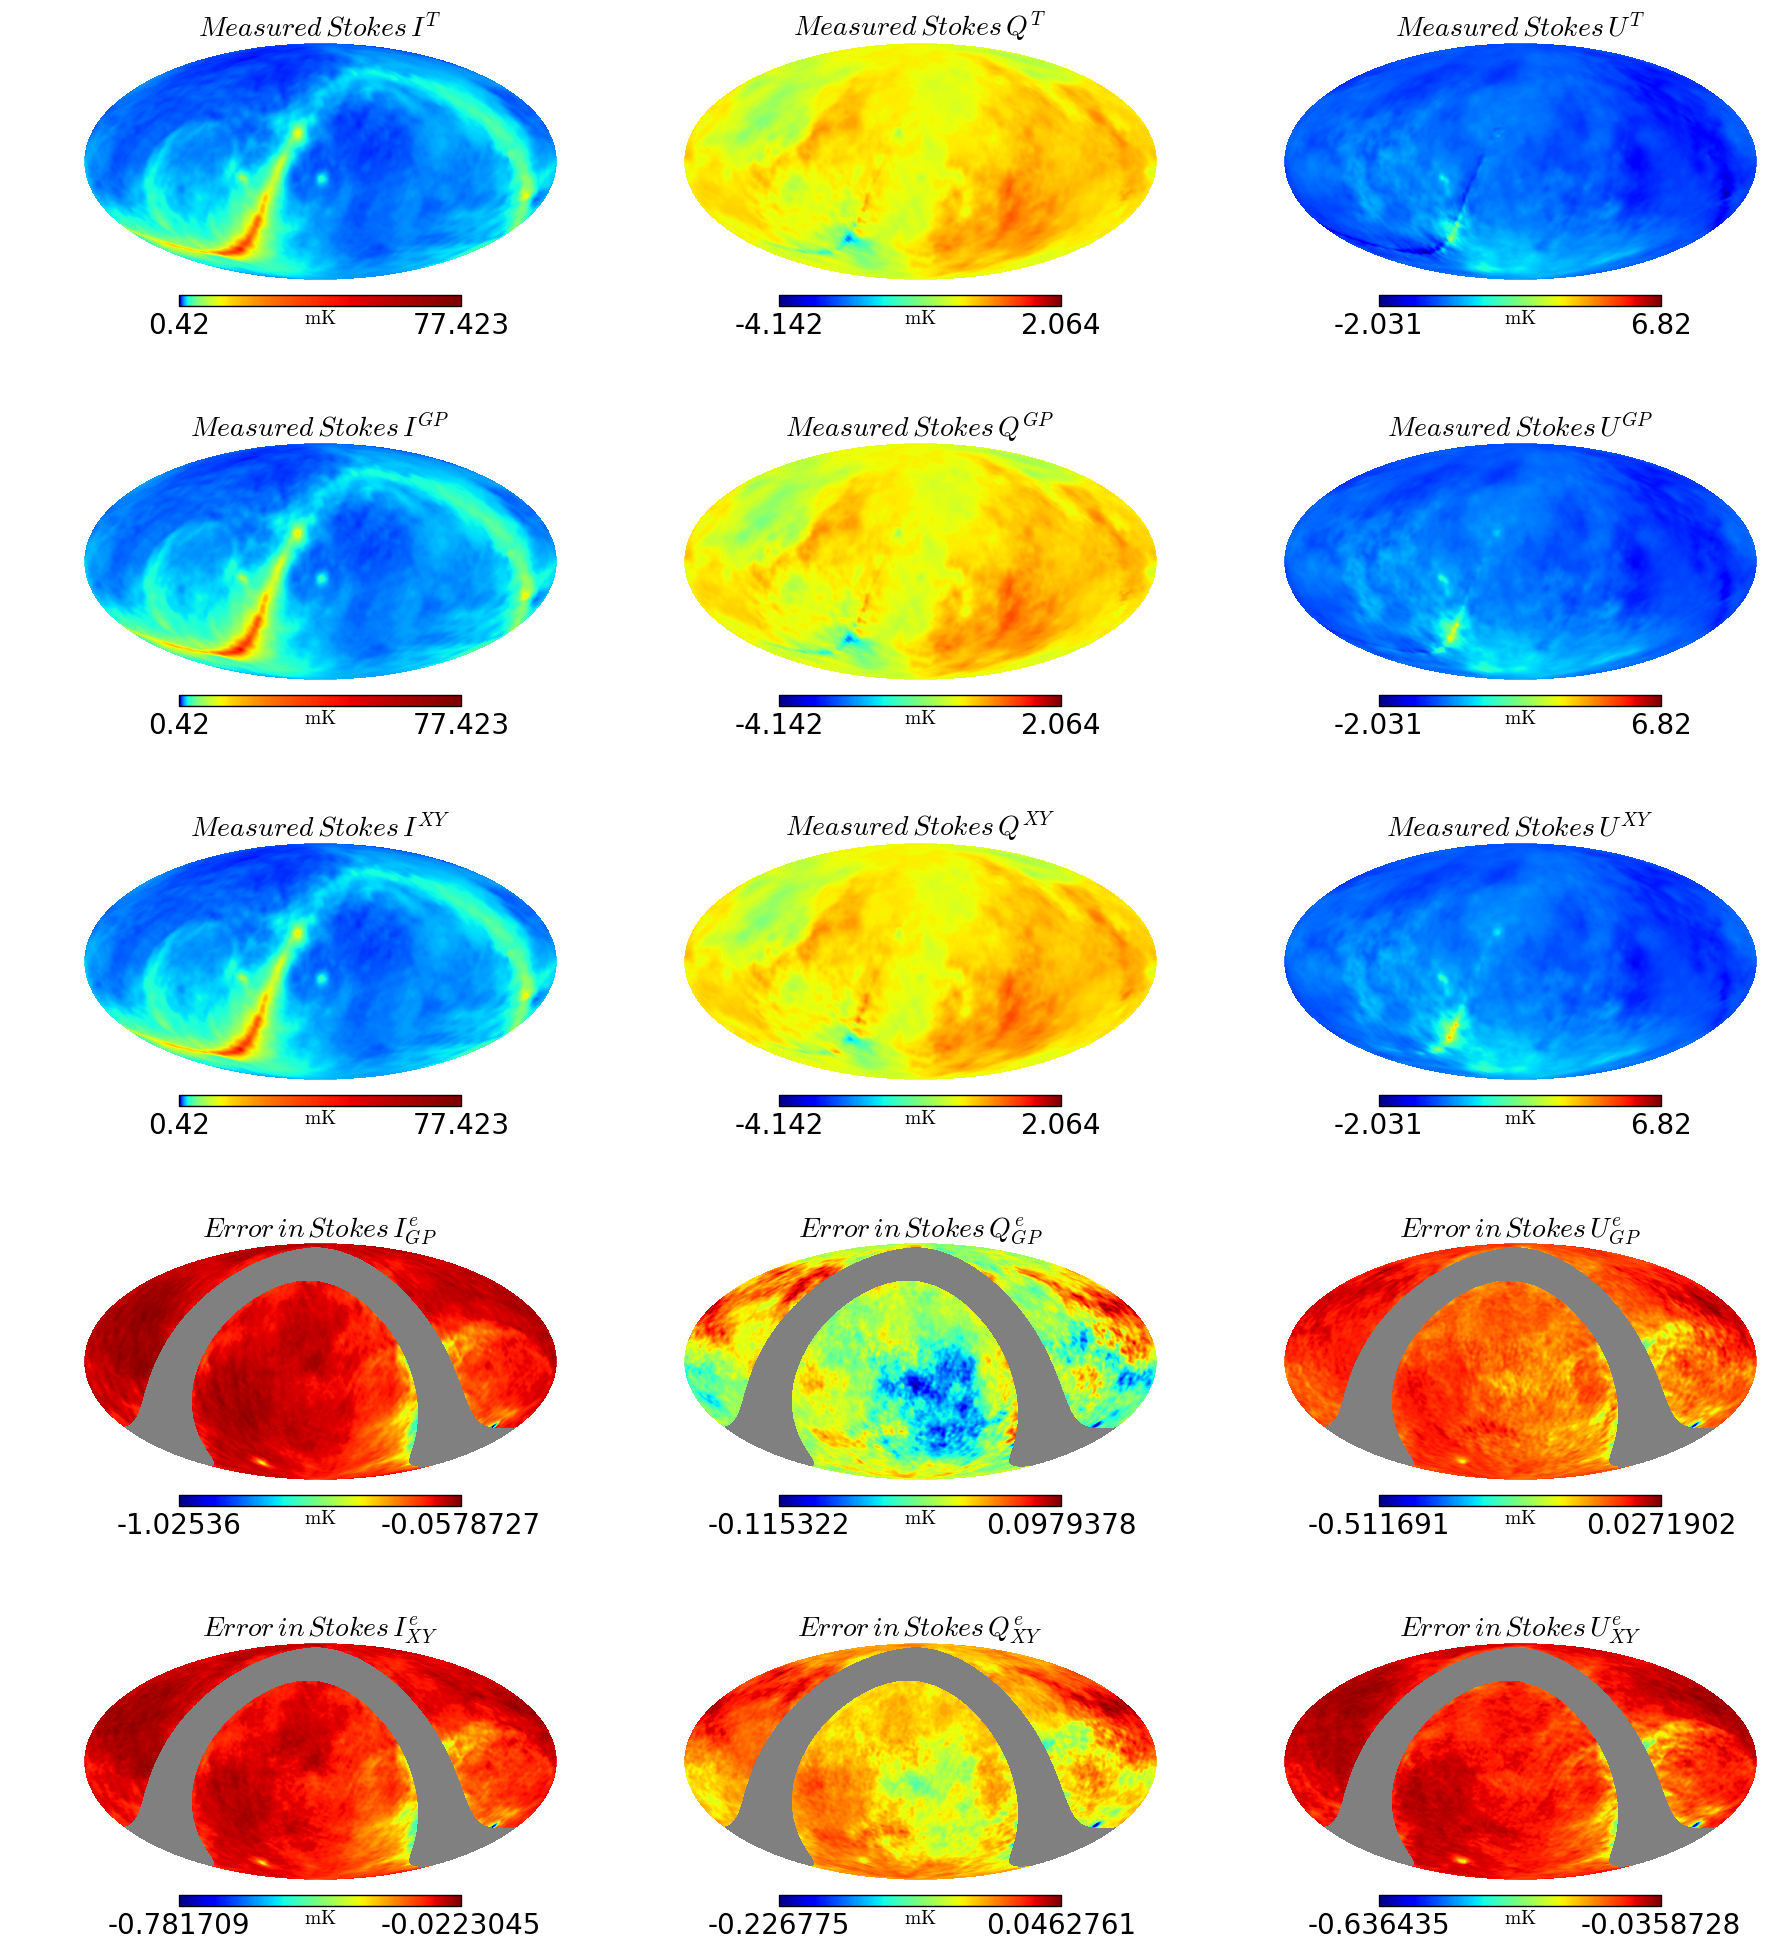
\includegraphics[width=6.6in]{sec3gp_conv/osk_ALL1}
    \end{minipage}
     \caption{The 1\textsuperscript{st} row maps depict the measured foregrounds of Stokes $I$, $Q$ and $U$ for using the non-distorted fully polarised beams in 
     Fig.~\ref{fig:truosk1} whilst the 2\textsuperscript{nd} and 3\textsuperscript{rd} rows represent the corrupted measured foregrounds due to gain and phase and dipole 
     orientation errors introduced into the beams respectively. The next two maps are the corresponding errors in $I$, $Q$ and $U$.}\label{fig:fgGP}
    \end{figure}
    \FloatBarrier
    %%    
The auto-power spectra presented in Fig.~\ref{fig:fg15} estimate the density of the measured foregrounds at different multipole moments. The first three rows in column $1$ show the respective power spectra plots of Stokes I, Q, U when we convolve the polarised foreground with true and gain and phase error beams produced from OSKAR. The next three rows in column $2$ represent the power spectra plots of Stokes I, Q, U respectively when we convolve the polarised foreground with true and dipole position error beams also produced from OSKAR. The last rows in the third column depict the respective power spectra plots of Stokes I, Q, U when we convolve the polarised foreground with two station beams of the JVLA. Note how the beam power in each plot of both OSKAR and the holographic measured beams is normalised to $1$. It is computed by finding the quotient of the power spectrum of the convolved sky map and the original sky map. In addition, note also in all cases, the PB effect of the convolved power spectrum.
The OSKAR beam power plots in Stokes $I$, $Q$ and $U$, converge at a multipole moment of $l=60$.
This value relates to an angular scale of $3.0^\circ$ on the sky whilst the power spectra of the VLA beams converge just at a multipole moment of $l=90$, giving an
angular scale of $2.0^\circ$ on the sky. The change in the value of multipole moments is because of different dish sizes which also results in producing different beamwidths. 
Furthermore, the angular scales computed are equivalent to the beam sizes used to convolve the original maps in Fig.~\ref{fig:f1000}. 
Note, even though we used two different aperture sizes for the simulation, the effect of these two PBs on the convolved power spectra of Stokes $I$, $Q$ and $U$ 
remains unaltered. This shows that in IM experiment, where we  measure the collective emission from many sources, smaller and relatively cheaper instruments can be used.
In this study, the measured values for the convolved power spectra of Stokes $I$, $Q$ and $U$ in both cases are $10\, \mathrm{mK^2}$, $0.1\, \mathrm{mK^2}$ 
and $0.1\, \mathrm{mK^2}$ respectively. Observe carefully how these values in Fig.~\ref{fig:fg15} actually predicted the foreground's temperature of the true sky.
Hence, the power spectrum of the corresponding errors in $I$, $Q$ and $U$ due to perturbation of the beams are $\approx$ $0.01\, \mathrm{mK^2}$, $10^{-4}\, \mathrm{mK^2}$ 
and $10^{-5}\, \mathrm{mK^2}$ respectively.
%%
%% I
  \begin{figure}
      \centering      
      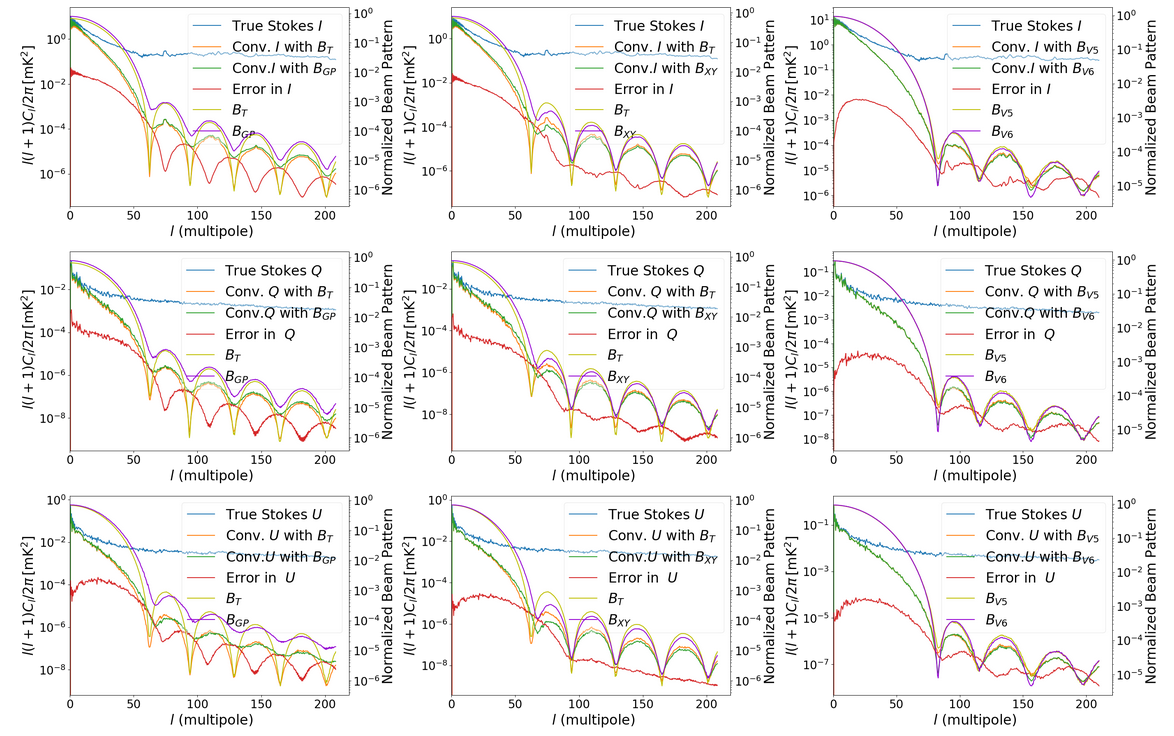
\includegraphics[width=6.8in]{powspectrum/fuck2}    
     \caption{Convolved angular power spectra  estimation of foreground maps. First row: Shows Stokes $I$ spectra plots for using simulated beams and holography measured beams. Second row: Displays Stokes $Q$ spectra plots for using simulated beams and holography measured beams. 
         Third row: Displays Stokes $U$ spectra plots for using simulated beams and holography measured beams.
          }\label{fig:fg15}   
    \end{figure}
    \FloatBarrier
 
% In either case, given the strength of the foregrounds in the galactic 
% centre we will not be able to recover scales less than that (i.e., $l<25$).
%%

% Next, we evaluate the systematic effects of beam errors in Stokes $I$, $Q$ and $U$. 
% 
% We then compute the standard errors of these residual plots to estimate the uncertainties in the angular power spectra when.
The spectra plots in Fig.~\ref{fig:sperr} depict the systematic effects of beam errors in Stokes $I$, $Q$ and $U$. These residual plots are measured as a result of the respective differences between the perturbed and true  measured full-sky maps. From the plots we can clearly observe that the systematic effects of beam errors between the simulated modelled beams and the holographic measurements   differ by 2 or 3 orders of mangitude with respect to the multipole moment ($l$). This is due to the uncertainties introduced in the power spectrum estimation for considering a notional beam over a measured beam.

Table~\ref{tbl:excel-table} shows the corresponding inaccuracies in the power spectrum estimation of Stokes $I$, $Q$ and $U$. It is computed as the standard deviations of the sampling distributions of the residual maps. Here, the residuals are determined as a result of the respective differences between the distorted and non-distorted convolved full-sky maps as reported in Fig.~\ref{fig:fgerr}. This is repeated for the systematic error maps (of using the JVLA holography beams) in Fig.~\ref{fig:B1}. For instance, the standard errors introduced in $Q \longrightarrow I$ are $\approx 0.015$ (due to gain and phase errors) and $0.014$ (due to the main dish surface orientation errors). Also, that of $U \longrightarrow I$ are $\approx 0.005$  and $0.0045$ accordingly. 
% These errors are then used to estimate the imperfections in the simulation by 
% The uncertainties in the spectra plots are as a result of the inaccuracies on the surface of the modelled dish presented in Fig.~\ref{fig:err}.
%%


    %%
 \begin{figure}
\begin{minipage}[H]{\linewidth}
      \centering
      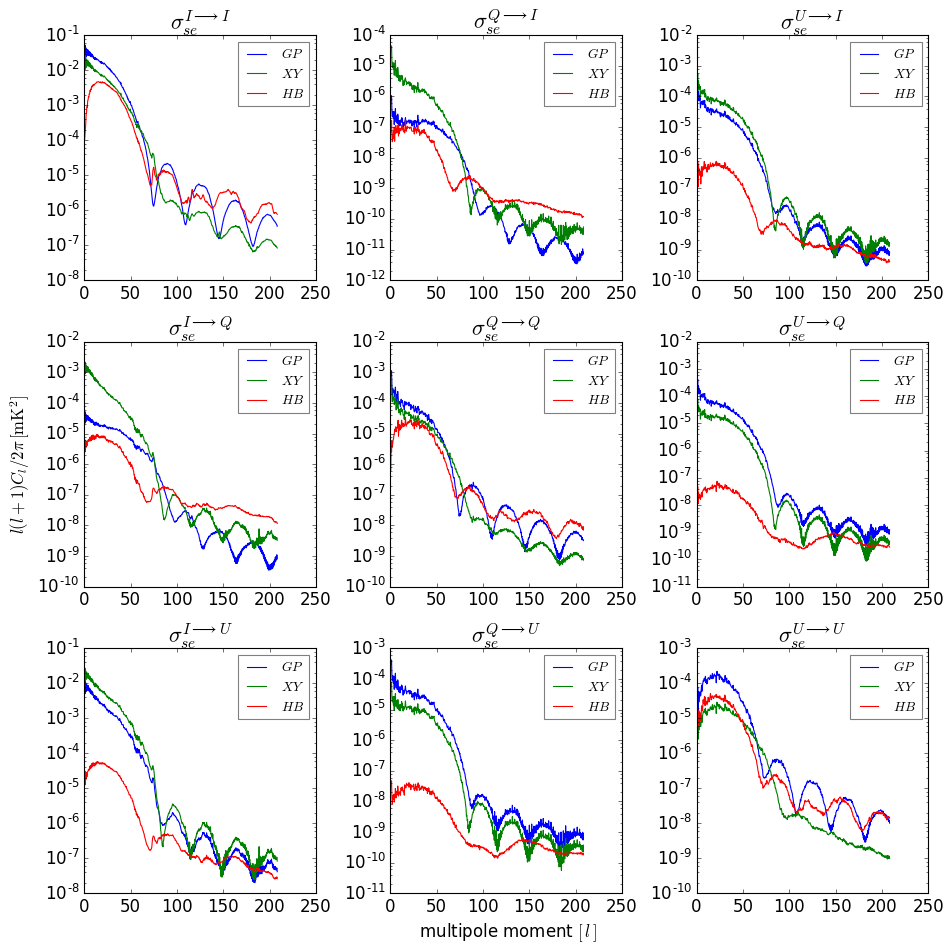
\includegraphics[width=6.6in]{powspectrum/osk_errplots}
      \end{minipage}
    \caption{These are the spectra plots of the systematic errors as shown in Fig.~\ref{fig:fgerr}. 
   The notations $GP$ and $XY$ in the legends denote the residuals for gain-phase and surface orientation errors in the simulated modelled beams, that of $HB$ depicts the errors  in the holography beams. These errors are then used to estimate the imperfections in the simulation by computing the expected value of the standard deviations of the sampling distributions of the residual maps to produce Table~\ref{tbl:excel-table}.}\label{fig:sperr}
\end{figure}
\FloatBarrier
% 
\begin{table}[H]\centering
\caption{Error introduced in the power spectrum estimation} 
\label{tbl:excel-table}
% \ra{1.1}
\begin{tabular}{@{}rrrcrrcrrcrr@{}}\toprule
& \multicolumn{2}{c}{$\bm{I}$} & \phantom{abc}& \multicolumn{2}{c}{$\bm{Q}$} & \phantom{abc} & \multicolumn{2}{c}{$\bm{U}$} & \phantom{abc} & \multicolumn{2}{c}{$\bm{TOTAL}$}\\
\cmidrule{2-3}  \cmidrule{5-6} \cmidrule{8-9} \cmidrule{11-12}
 & $GP $ & $XY $ && $GP$ & $XY $  && $GP $ & $XY $  && $GP$ & $XY $ \\ \midrule
% & GP $ & $ XY $ && $ GP  $ & $ XY $  && $ GP $ & $ XY $  && $ GP $ & $ XY $ \\ \midrule
{}\\
$\bm{I}$ & 0.0640 & 0.0640 && 0.0151 & 0.0137  && 0.0050 & 0.0045 && \textbf{0.0841} & \textbf{0.0822}\\
$\bm{Q}$ & 0.0010 & 0.0008 && 0.0221 & 0.0224 && 0.0007 & 0.0055 && \textbf{0.0238} & \textbf{0.0287}\\
$\bm{U}$ & 0.0007 & 0.0007 && 0.0194 & 0.0341 && 0.0354 & 0.0362  && \textbf{0.0555} & \textbf{0.0710}\\
\bottomrule
\end{tabular}
%\caption{Caption}
\end{table}
 \FloatBarrier     

In IM experiments, the HI signal is measured in Stokes $I$, so we are particularly interested in the total intensity and the leakages from polarization 
into Stokes $I$ (that is, $|Q + iU| \longrightarrow I$). Fig.~\ref{fig:lk} shows how the $|Q + iU| \longrightarrow I$  and the error in Stokes $I$ map affect the HI signal. 
Here, a spherical power spectrum of the simulated model of $21\, \mathrm{cm}$  brightness temperature at $z \approx 0.67$ produced from the 
CRIME\footnote{{\tt http://intensitymapping.physics.ox.ac.uk/CRIME.html}} fast simulation software and described by \citep{2014MNRAS.444.3183A} 
is generated and then compared with the spectra plots of the  Galactic foregrounds. % presented in Figs.~\ref{fig:lk1} and~\ref{fig:lk2}. 
The HI signal power in the right side of the plot is higher than the $|Q + iU| \longrightarrow I$ at a multipole moment of $l=100$ which is about $4$ orders of magnitude greater at lower scales. 
This occurs when we do not correct the beam errors (i.e., gain, phase and orientation) in Stokes $I$ at all. 
The fractional leakage of $|Q + iU|/I$ is computed to give $\approx 1.0 \%$ for the intrinsic case (i.e., $|Q + iU|_{\rm T}$) where a true model of the beam is known.
The spectra plots reported in the other plot, try to correct the columns that feeds into Stokes $I$ (i.e., $Q \longrightarrow I$, $U \longrightarrow I$ and $I \longrightarrow I$)
by assuming the corresponding beams (i.e., $m_{\rm QI}$, $m_{\rm UI}$ and $m_{\rm II}$) are not known to the extent to which they have been assumed in this paper. In this case,
the power spectrum of the HI signal can be observed at a multipole moment of $l=25$.
We conclude that if the knowledge of the beam is of a similar quality than the one assumed in this paper, then we will be able to recover the cosmological HI signal 
without great problems and without further calibration on scales larger than $l = 100$. However, this work suggests that if polarization calibration is performed correctly 
then results can be improved and we can recover scales above $l=25$. 
%%
\begin{figure}
\centering    
    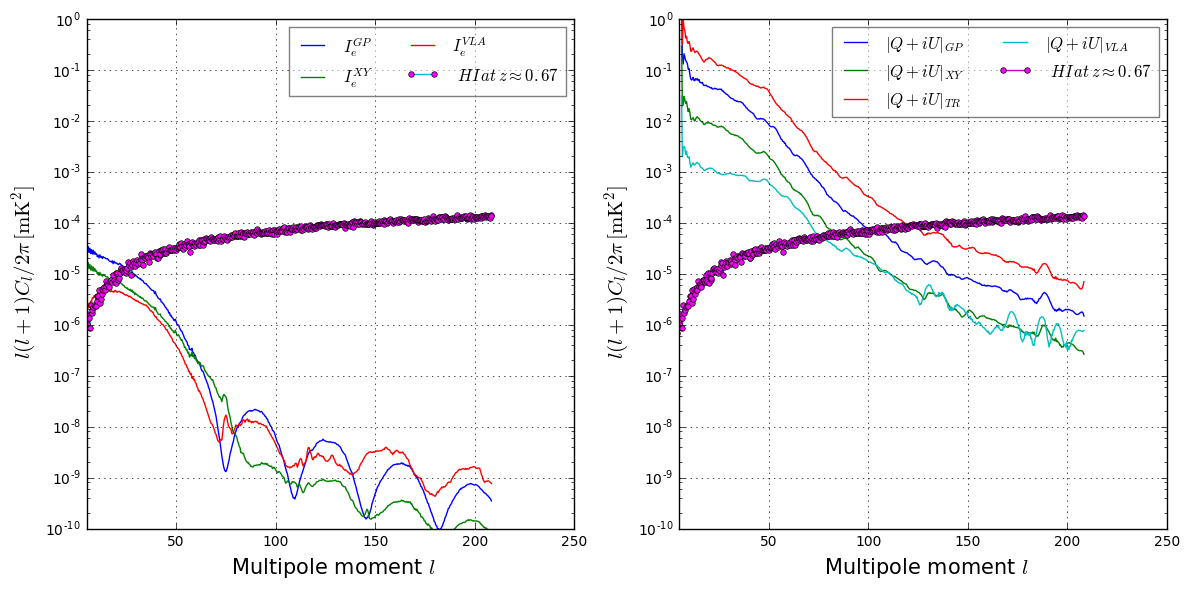
\includegraphics[width=\linewidth]{powspectrum/hisim}
 \caption{The spectra plots compare the effect of recovering the cosmological $21\, \mathrm{cm}$ signal by calibrating for the beam errors in Stokes $I$ 
  to when there is no beam correction at  all. The solid circular spectrum is the simulated $21\, \mathrm{cm}$ 
  brightness temperature described by \citep{2014MNRAS.444.3183A} at a $z\approx 0.67$. 
  LEFT SIDE PLOT: Here, we show how to estimate the $21\, \mathrm{cm}$ signal when we correct the errors in Stokes $I$.         
  RIGHT SIDE PLOT: We quantify the amount of leakages into Stokes $I$ when we do not perform any beam correction.
  The spectrum $ (|Q + iU|_{T} )$, is the intrinsic leakage in $I$ when we adopt true modelled beams as shown in  Fig.~\ref{fig:truosk1}.
  The other plots $( |Q + iU|_{GP}, |Q + iU|_{XY} , |Q + iU|_{VLA})$  are the leakages in $I$ when we use perturbed modelled beams (i.e., gain, phase and main dish surface orientation errors) and holography measured beams respectively.}\label{fig:lk}
 \end{figure} 
 \FloatBarrier

 
%     
\section{Conclusions} \label{sec:conclusions}
%%
The study introduces an application of the OSKAR software as a relatively cheap technique to produce realistic PBs and perturbations
(using gain, phase, and main dish surface orientation errors) for IM experiments. These fully polarized modelled beams are then
used to simulate the full-sky polarization maps by the method of convolution in order to compute the intensities of the diffuse
Galactic foregrounds and determine the amount of signal that has seeped from linear polarization into total intensity. The simulation is
repeated using the holography-measured beams and then compared with the modelled beams in order to estimate the error introduced in
the power spectrum when modelled beams are used. The following are the key findings of the research:

\begin{itemize}
\item We use $80 000$ dipoles to model the distribution of the dish-like surface of the antenna. This produces $\approx 0.10$ per cent perturbed
inaccuracies on the dish surface due to the random placement of the dipoles, which are not exactly phased up. The value of the perturbed
inaccuracies will increase if the number of dipoles is $\ll 80 000$.
%%
\item The perturbed inaccuracies due to the imperfections in the nominal orientation of the dipoles introduce fractional errors of
$0.08 \%$ for Stokes $I$, $0.03 \%$ for $Q$ and $0.07 \%$ for $U$ in the convolved power spectrum estimation. 
Note that these occur when we assume to use modelled beams whilst we convolve the foregrounds with measured beams.
%%
\item Furthermore, if we construct a model of a beam and then carry out polarization rotation and calibration of the phase in order
to correct the beam in Stokes $I$, then the power of the HI signal can be estimated at a multipole moment of $l = 25$. But, if we don’t do
any correction at all for the beam, then the power spectrum of the HI signal is measured at a multipole moment of $l=100$. This makes
the latter multipole moment be $\approx 4$ orders of magnitude higher than when we correct the error in the beam.

\item Finally, if a true model of the beam is assumed, then the intrinsic fractional leakage of $|Q + iU|_{\rm T} \longrightarrow I$ is $\approx 1.0$ percent.
\end{itemize}
%%
\noindent  To recap, we have shown that the {\tt oskar} package can simulate the beam patterns and as well as distortions of the dish. The model we adopted to do this, is to 
create a dense set of dipole orientations that imitate the aperture illumination patterns of the dish, with full blockage from the quad leg structure and other supporting frame.
The convolution technique has shown to be a good mathematical model to use for measuring the intensity of the foreground. Hence, for a full polarization model 
of the beams, we can  actually measure the fractional leakages we are instereted in. For the next chapter, we extend this simulation technique to investigate HI intensity mapping 
with MeerKAT L-band beams. 
%%
